\documentclass[conference]{IEEEtran}
\IEEEoverridecommandlockouts

\usepackage{cite}
\usepackage{amsmath,amssymb,amsfonts}
\usepackage{graphicx}
\usepackage{textcomp}
\usepackage{xcolor}
\usepackage{booktabs}
\usepackage{multirow}
\usepackage{array}

\def\BibTeX{{\rm B\kern-.05em{\sc i\kern-.025em b}\kern-.08em
    T\kern-.1667em\lower.7ex\hbox{E}\kern-.125emX}}

\begin{document}

\title{SAGAM: Interpretable Nonlinear Survival Stacking for Lung
Adenocarcinoma Prognosis}

\author{
\IEEEauthorblockN{Anonymous Author(s)}
\IEEEauthorblockA{Submitted for blind review}
}

\maketitle

% ============================================================
\begin{abstract}
Accurate lung adenocarcinoma (LUAD) prognosis remains challenging because
survival models vary in reliability across cohorts and risk ranges.
Existing survival stacking methods combine base learner predictions using
scalar linear weights, which cannot capture nonlinear or score-range-dependent
relationships between model predictions and patient hazard.
We propose \textbf{SAGAM}, an interpretable survival stacking framework
that represents each base learner's contribution as a smooth cubic B-spline
function of its out-of-fold risk score within a regularized Cox proportional
hazards model.
On TCGA-LUAD (n\,=\,501, 181 events) under strict five-fold nested
cross-validation with leakage-controlled preprocessing and fold-specific
feature selection, SAGAM achieves the highest concordance index among all
stacking-based approaches (0.634\,$\pm$\,0.050), outperforms linear Cox
stacking in four of five folds, and produces significant patient risk
stratification ($p = 6.94 \times 10^{-5}$).
External validation on two independent GEO cohorts reveals stage-dependent
generalization: on GSE31210 (226 stage~I/II patients, 35 events), SAGAM's
advantage grows from $+0.006$ (internal) to $\mathbf{+0.086}$, with
significant cross-cohort risk stratification ($p = 0.030$); on
GSE68465 (432 all-stage patients, 226 events), SAGAM does not outperform
linear stacking ($\Delta\!=\!-0.026$, NS), consistent with the internal
subgroup finding that SAGAM's benefit is largest in Stage~I/II where base
learner performance is heterogeneous and molecular features may contribute
to nonlinear model behavior, although incremental discrimination beyond
AJCC staging is not demonstrated in this study.
AJCC stage-only Cox remains the strongest internal discriminator
(0.657\,$\pm$\,0.044), confirming the dominant prognostic role of clinical
staging; SAGAM is therefore best understood as an interpretable nonlinear
stacking mechanism that improves over scalar-weighted ensembles and exposes
model-specific contribution functions, rather than a universal replacement
for clinical staging or neural survival models.
\end{abstract}

\begin{IEEEkeywords}
survival analysis, lung adenocarcinoma, generalized additive model,
ensemble stacking, interpretability, nested cross-validation, TCGA
\end{IEEEkeywords}

% ============================================================
\section{Introduction}
% ============================================================

Lung adenocarcinoma (LUAD) is the most prevalent histological subtype of
non-small cell lung cancer and the leading cause of cancer mortality
worldwide, with approximately 508,000 deaths annually~\cite{sung2021global}.
AJCC pathological stage is the dominant clinical predictor of survival,
yet machine learning models can capture complementary prognostic signals
from molecular, genomic, and transcriptomic features that staging
alone cannot express~\cite{cancer2014comprehensive}.

A growing body of work applies diverse survival learners to TCGA-LUAD:
random survival forests (RSF)~\cite{ishwaran2008random}, gradient boosting
survival analysis (GBS)~\cite{hothorn2006survival}, XGBoost with a Cox
objective~\cite{chen2016xgboost}, and deep neural approaches such as
DeepSurv~\cite{katzman2018deepsurv}.
Each family captures different aspects of the survival structure, and no
single learner consistently dominates across datasets~\cite{binder2009boosting}.
This motivates ensemble stacking~\cite{van2007super}, which trains a
meta-learner on out-of-fold (OOF) predictions to exploit complementary
strengths.

The critical design choice in stacking is the meta-learner.
All published survival stacking methods use \emph{linear} meta-learners:
IPCW-weighted combinations~\cite{lyu2026supersurv,golmakani2024joint},
non-negative Bayesian
optimization~\cite{zhao2024bayesian}, and regularized linear Cox regression
on raw risk scores~\cite{vock2016adapting}.
A linear meta-learner assigns each base model a fixed scalar weight,
implicitly assuming uniform contribution across all patient risk levels.
This assumption is problematic: a model may be well-calibrated for low-risk
patients but unreliable at extreme risk scores, or its relationship to
the true hazard may be nonmonotone.
A single global coefficient cannot express such score-range-dependent
reliability.

We address this with \textbf{SAGAM}, which replaces scalar weights with
smooth nonlinear functions of base learner risk scores:
\begin{equation}
  h(t \mid \mathbf{x}) = h_0(t)
    \exp\!\Bigl(\sum_{k=1}^{K} f_k\!\bigl(\hat{\theta}_k(\mathbf{x})\bigr)\Bigr),
  \label{eq:sagam}
\end{equation}
where $\hat{\theta}_k(\mathbf{x})$ is the OOF risk score from base
learner $k$ and $f_k(\cdot)$ is a smooth function parameterized by a
cubic B-spline basis.
This formulation allows the meta-learner to learn score-range-dependent
integration rules, providing greater expressiveness than linear stacking
and interpretability through the smooth contribution plots $f_k$.

SAGAM's contribution is not that it surpasses AJCC staging or neural
survival models in raw discrimination---it does not.
Rather, SAGAM addresses a methodological gap: existing survival stacking
approaches use scalar linear weights, whereas SAGAM provides interpretable
nonlinear score-range-dependent model integration through a smooth GAM
meta-learner.

\textbf{Contributions:}
\begin{enumerate}
  \item \textbf{Method:} To the best of our knowledge, SAGAM is the
    first survival stacking framework to use GAM-style smooth B-spline
    functions of base learner risk scores as the Cox meta-learning mechanism,
    distinct from prior work (CoxNAM~\cite{coxnam2023}, CRISP-NAM~\cite{crispnam2025})
    that applies smooth functions to raw covariates within a single model.
  \item \textbf{External validation:} The SAGAM advantage over
    linear stacking grows from $+0.006$ (internal) to $+0.086$ on GSE31210,
    a large external increase consistent with the score-range-dependent
    integration hypothesis, although the GSE68465 result ($\Delta\!=\!-0.026$)
    shows this benefit is cohort-dependent rather than universal.
  \item \textbf{Interpretability and nonlinearity validation:} The smooth
    functions $f_k$ expose score-range-dependent contributions quantified
    by per-learner nonlinearity analysis; all four base learners show
    substantial deviation from linearity, justifying the B-spline design.
  \item \textbf{Honest evaluation:} Five-fold nested CV with fold-specific
    preprocessing, gene selection, and feature selection; clinical Cox
    baselines including stage-only Cox; Stage~+~SAGAM incremental tests;
    IBS and Ctd-AUC metrics; and full spline df sensitivity analysis
    provide complete methodological context.
  \item \textbf{Best stacking performance:} SAGAM achieves the highest
    C-index (0.634), lowest IBS (0.177), and highest Ctd-AUC (0.650) among
    stacking-based approaches; 73.9\% of bootstrap resamples favor SAGAM
    over linear stacking on C-index, and 93.8\% on IBS.
    Significant risk stratification ($p = 6.94 \times 10^{-5}$) and
    subgroup analysis show the largest advantage in Stage~I/II
    ($\Delta\!=\!+0.010$) where base learner performance is most heterogeneous.
\end{enumerate}

% ============================================================
\section{Related Work}
% ============================================================

\subsection{Survival Models for LUAD}

Published TCGA-LUAD concordance indices using pre-treatment features range
from 0.62 to 0.73~\cite{astley2022lung,he2024immune}.
He~et~al.~\cite{he2024immune} report C-index 0.716 using immune and
metabolic gene signatures.
Higher values incorporate post-treatment predictors~\cite{bartholomai2019survival}
unavailable at diagnosis.
Multi-omics autoencoder approaches achieve C-index 0.65~\cite{chen2020multiomics}.

\subsection{Survival Ensemble Stacking}

Stacking~\cite{van2007super} trains a meta-learner on cross-validated base
model predictions.
In survival analysis, all published meta-learners are \textbf{linear}.
SuperSurv~\cite{lyu2026supersurv} (concurrent preprint) provides a unified
R framework using IPCW-weighted linear combinations.
The joint survival super learner~\cite{golmakani2024joint} selects the best
single model via Integrated Brier Score.
Non-negative Bayesian stacking~\cite{zhao2024bayesian} applies linear
combinations for high-dimensional omics.
A two-stage heterogeneous stacking~\cite{huang2023twostage} uses linear
Cox regression as the meta-learner.
An interpretable stacking ensemble for lung cancer~\cite{effective2024lung}
employs SHAP for post-hoc interpretation but retains a linear meta-learner.
To the best of our knowledge, SAGAM is the first to replace scalar weights with smooth nonlinear functions.

\subsection{GAMs and Splines in Survival Analysis}

GAMs~\cite{hastie1990gam} model responses through smooth additive functions.
Spline terms in Cox-PH are established for nonlinear covariate
effects~\cite{therneau2000modeling}.
CoxFNN~\cite{coxfnn2024} uses neural networks for nonlinear covariate effects.
CoxNAM~\cite{coxnam2023} and CRISP-NAM~\cite{crispnam2025} use Neural
Additive Models within the Cox hazard to learn interpretable nonlinear
covariate effects for single-model survival prediction.
Coxmos~\cite{coxmos2025} extends Cox models for high-dimensional multi-omics.
These methods apply smooth functions to \emph{raw covariates} within a
single model.
SAGAM applies smooth functions to \emph{base learner risk scores} as
the meta-learning mechanism for ensemble stacking---a conceptually and
technically distinct contribution that enables score-range-dependent
integration of multiple pre-trained survival models.

\subsection{Related Work Comparison}

Table~\ref{tab:related} shows that SAGAM uniquely combines survival
stacking with nonlinear, interpretable meta-learning and external
validation.

\begin{table}[t]
\caption{Comparison of Survival Stacking Approaches}
\label{tab:related}
\begin{center}
\setlength\tabcolsep{3pt}
\begin{tabular}{lcccc}
\toprule
\textbf{Method} & \textbf{Stack} & \textbf{Nonlin.} & \textbf{Interp.} & \textbf{Ext.}\\
\midrule
Joint surv. SL~\cite{golmakani2024joint}  & \checkmark & -- & -- & --\\
Bayes. stacking~\cite{zhao2024bayesian}   & \checkmark & -- & -- & --\\
Two-stage~\cite{huang2023twostage}        & \checkmark & -- & -- & --\\
SuperSurv~\cite{lyu2026supersurv}         & \checkmark & -- & -- & --\\
DeepSurv~\cite{katzman2018deepsurv}       & --  & \checkmark & -- & sometimes\\
\textbf{SAGAM (ours)}    & \checkmark & \checkmark & \checkmark & \checkmark\\
\bottomrule
\end{tabular}
\end{center}
\end{table}

% ============================================================
\section{Methods}
% ============================================================

\subsection{Dataset and Features}

We use the TCGA-LUAD PanCan Atlas 2018 cohort from
cBioPortal~\cite{cerami2012cbio}: \textbf{501 patients}, \textbf{181 OS
events} (36.1\%), overall survival from initial pathologic diagnosis to
death in months.
We apply comprehensive leakage prevention, removing 34 column types
including all post-diagnosis outcome variables, temporal follow-up fields,
and administrative identifiers.

We define four feature groups of increasing complexity:
\begin{itemize}
  \item \textbf{Stage-only:} AJCC T, N, M, and overall pathological stage.
  \item \textbf{Clinical:} Stage plus age, sex, grade, race, ethnicity,
    prior diagnosis, radiation therapy, weight.
  \item \textbf{Genomic:} Aneuploidy Score, TMB (nonsynonymous), Tumor
    Break Load, MSI MANTIS Score, MSIsensor Score.
  \item \textbf{Hypoxia:} Buffa, Winter, and Ragnum mRNA-derived hypoxia
    scores~\cite{buffa2010hypoxia}.
\end{itemize}
The full feature set combines all four groups.
Additionally, in each outer fold, the top-5 mRNA-derived genes (by
univariate concordance index on outer-training data only) are added as
transcriptomic features.
Binary missing-data indicators are included for features with $>15\%$
missingness.

\subsection{Five-Fold Nested Cross-Validation}

A single 80/20 train/test split on n\,=\,501 yields $\approx$36 test
events per fold (SE\,$\approx$0.07 per fold), making single-split C-index
estimates unreliable.
We employ \textbf{stratified five-fold nested cross-validation}.
In each outer fold:
\begin{enumerate}
  \item Outer split stratified by event status.
  \item All preprocessing (imputation, encoding, scaling) fitted on
    outer-training data.
  \item mRNA gene selection and CoxNet feature selection performed via
    inner 3-fold CV on outer-training data.
  \item RSF, GBS, XGBoost, and DeepSurv trained via inner 5-fold OOF;
    OOF risk scores collected.
  \item B-spline meta-feature matrix $\mathbf{M}$ constructed; SAGAM and
    linear stacking both tuned on a 20\% inner-validation split.
  \item All models evaluated on the held-out outer-test fold.
\end{enumerate}
Pooled OOF predictions across all five folds (n\,=\,501) are used for
Kaplan-Meier analysis.

\subsection{Cox Baselines}

To provide clinical context, we run CoxNet baselines using each of the
four feature groups under the same 5-fold stratified CV.
The stage-only Cox establishes a strong single-variable reference consistent
with AJCC staging's dominant role in LUAD prognosis.

\subsection{SAGAM Meta-Learner}

Each base learner's OOF risk scores are expanded into a B-spline basis:
\begin{equation}
  \mathbf{B}_k = \mathrm{bs}\!\bigl(\hat{\boldsymbol{\theta}}_k^{\text{OOF}};\;
    \text{df}\!=\!4,\;\text{degree}\!=\!3\bigr) \in \mathbb{R}^{n \times 4}.
  \label{eq:spline}
\end{equation}
The meta-feature matrix $\mathbf{M} = [\mathbf{B}_1 \mid \cdots \mid
\mathbf{B}_4] \in \mathbb{R}^{n \times 16}$ is fitted with CoxNet
($\ell_1$ ratio 0.9):
\begin{equation}
  \hat{h}(t \mid \mathbf{x}) = h_0(t)\,\exp\!\bigl(\mathbf{M}\hat{\boldsymbol{\beta}}\bigr).
  \label{eq:cox}
\end{equation}
The smooth contribution of learner $k$ is:
$f_k(s) = \mathbf{b}_k(s)^\top \hat{\boldsymbol{\beta}}_k$.
We select $\text{df}\!=\!4$ via ablation (Table~\ref{tab:df_ablation}).
Test-time predictions are clipped to the training score range.

\subsection{Linear Cox Stacking Baseline}

CoxNet is fitted directly on the four raw OOF risk scores (no splines):
\begin{equation}
  h_{\text{lin}}(t \mid \mathbf{x}) =
    h_0(t)\exp\!\bigl(\boldsymbol{\gamma}^\top\hat{\boldsymbol{\theta}}\bigr).
\end{equation}
The C-index difference SAGAM$-$Linear provides empirical evidence that
nonlinear smooth weighting can add value over scalar linear combination.

\subsection{External Validation}

SAGAM is trained on all 501 TCGA patients using transferable features
(clinical stage, age, sex, top-10 mRNA genes by TCGA univariate concordance
index) and applied to two independent GEO cohorts.
\textbf{GSE31210} (Takeuchi et al.): 226 pure LUAD, stage I/II,
35 OS events, median follow-up 57.3 months (GPL570 array).
All 10 selected mRNA genes (DKK1, FAM83A, RHOV, IRX5, SFTA3, CD1B,
PKP2, TNS4, LYPD3, TFAP2A) are present in the GSE31210 Affymetrix array.
\textbf{GSE68465} (Director's Challenge Consortium): 432 LUAD patients
across all disease stages, 226 OS events (GPL96 array).
For GSE68465, the transferable feature set included age, sex, and the
TCGA-selected mRNA genes; AJCC stage was not sufficiently harmonized for
stage-only Cox evaluation on this cohort.
Because platform differences and cohort composition restrict complete
feature matching, external results are interpreted as transportability
assessments rather than direct clinical deployment validation.
External preprocessing (imputation, scaling) uses TCGA training-set
statistics exclusively for both cohorts.

\subsection{Hyperparameters}

Table~\ref{tab:hyperparams} summarizes all fixed hyperparameters.

\begin{table}[t]
\caption{Model Hyperparameters}
\label{tab:hyperparams}
\begin{center}
\begin{tabular}{ll}
\toprule
\textbf{Component} & \textbf{Settings} \\
\midrule
RSF        & 300 trees; $\sqrt{p}$ features; min 5 leaves \\
GBS        & 300 rounds; lr 0.05; max depth 3 \\
XGBoost    & \texttt{survival:cox}; $\eta$=0.05; depth 3; sub. 0.8 \\
DeepSurv   & 64-32-1 MLP; ReLU; dropout 0.3; Adam $10^{-3}$ \\
CoxNet FS  & $\ell_1$=0.9; $\alpha\in[10^{-2},10^2]$ (12 vals) \\
SAGAM      & cubic B-spline; df=4; CoxNet $\ell_1$=0.9 \\
\bottomrule
\end{tabular}
\end{center}
\end{table}

\subsection{Statistical Testing}

We report bootstrap confidence intervals (1,000 resamples) for all C-index
estimates and for differences between SAGAM and each comparator.
Fold-level pairwise comparisons use the Wilcoxon signed-rank test (n=5 folds;
minimum achievable one-sided $p$ is 0.0625).

% ============================================================
\section{Results}
% ============================================================

\subsection{Cox Baselines and Internal Discrimination}

Table~\ref{tab:baselines} shows all models under 5-fold nested CV.

\begin{table}[t]
\caption{Full Performance Comparison — TCGA-LUAD 5-Fold Nested CV
(n\,=\,501). Stage-only Cox achieves the highest mean C-index; SAGAM
achieves the best stacking performance with lowest variance.}
\label{tab:baselines}
\begin{center}
\begin{tabular}{llcc}
\toprule
\textbf{Type} & \textbf{Model} & \textbf{Mean C} & \textbf{Std} \\
\midrule
\multirow{5}{*}{\parbox{1cm}{Cox\\baselines}}
& Stage-only Cox & \textbf{0.657} & 0.044 \\
& Clinical-only Cox & 0.646 & 0.028 \\
& Clin.+Genomic Cox & 0.641 & 0.032 \\
& All-features CoxNet & 0.641 & 0.032 \\
& Stage + SAGAM risk & 0.653 & 0.037 \\
\midrule
\multirow{4}{*}{\parbox{1cm}{Base\\learners}}
& RSF~\cite{ishwaran2008random}        & 0.619 & 0.052 \\
& GBS~\cite{hothorn2006survival}       & 0.605 & 0.066 \\
& XGBoost-Cox~\cite{chen2016xgboost}   & 0.602 & 0.053 \\
& DeepSurv~\cite{katzman2018deepsurv}  & 0.636 & 0.058 \\
\midrule
\multirow{2}{*}{Stacking}
& Linear Cox Stacking    & 0.627 & 0.055 \\
& \textbf{SAGAM (ours)}  & \textbf{0.634} & \textbf{0.050} \\
\midrule
\multicolumn{4}{l}{\small Pooled OOF: SAGAM 0.625; Linear 0.618} \\
\bottomrule
\end{tabular}
\end{center}
\end{table}

Four findings emerge from Table~\ref{tab:baselines}.

\textbf{First}, stage-only Cox (0.657) achieves the highest overall mean
C-index, confirming the dominant role of AJCC staging in LUAD prognosis.
This is consistent with the clinical literature: stage captures tumor
burden, nodal involvement, and metastatic spread at diagnosis.

\textbf{Second}, adding clinical, genomic, and hypoxia features to a Cox
model does not improve over stage-only (decreases from 0.657 to 0.641),
consistent with the curse of dimensionality in penalized linear models
when the dominant predictor is already present.

\textbf{Third}, combining SAGAM risk scores with stage (Stage + SAGAM,
0.653) does not improve over stage-alone (0.657), indicating that SAGAM's
risk scores do not carry substantial incremental prognostic information
beyond AJCC staging.
This reinforces that SAGAM's contribution is methodological---providing
an interpretable nonlinear stacking framework---rather than clinical
superiority over traditional staging.

\textbf{Fourth}, among stacking-based methods, SAGAM (0.634) outperforms
linear Cox stacking (0.627) in four of five folds
($\Delta\!=\!+0.006$; Wilcoxon $p\!=\!0.313$; bootstrap CI
$[-0.013, +0.025]$) and achieves lower fold-to-fold variance (std 0.050
vs.\ 0.055 for linear stacking, 0.058 for DeepSurv).

\subsection{Performance Overview}

Fig.~\ref{fig:perf} summarizes mean\,$\pm$\,std concordance index for
all evaluated models.
SAGAM achieves the lowest variance across folds (std 0.050) among all
stacking methods, while the stage-only Cox baseline achieves the highest
mean.
The performance hierarchy---stage Cox $>$ DeepSurv $\approx$ SAGAM $>$
linear stacking $>$ other base learners---reveals an important structure:
AJCC staging dominates, nonlinear neural and GAM-based approaches form a
competitive second tier, and simple linear ensembles rank below their
best constituent models.

\begin{figure}[t]
  \centerline{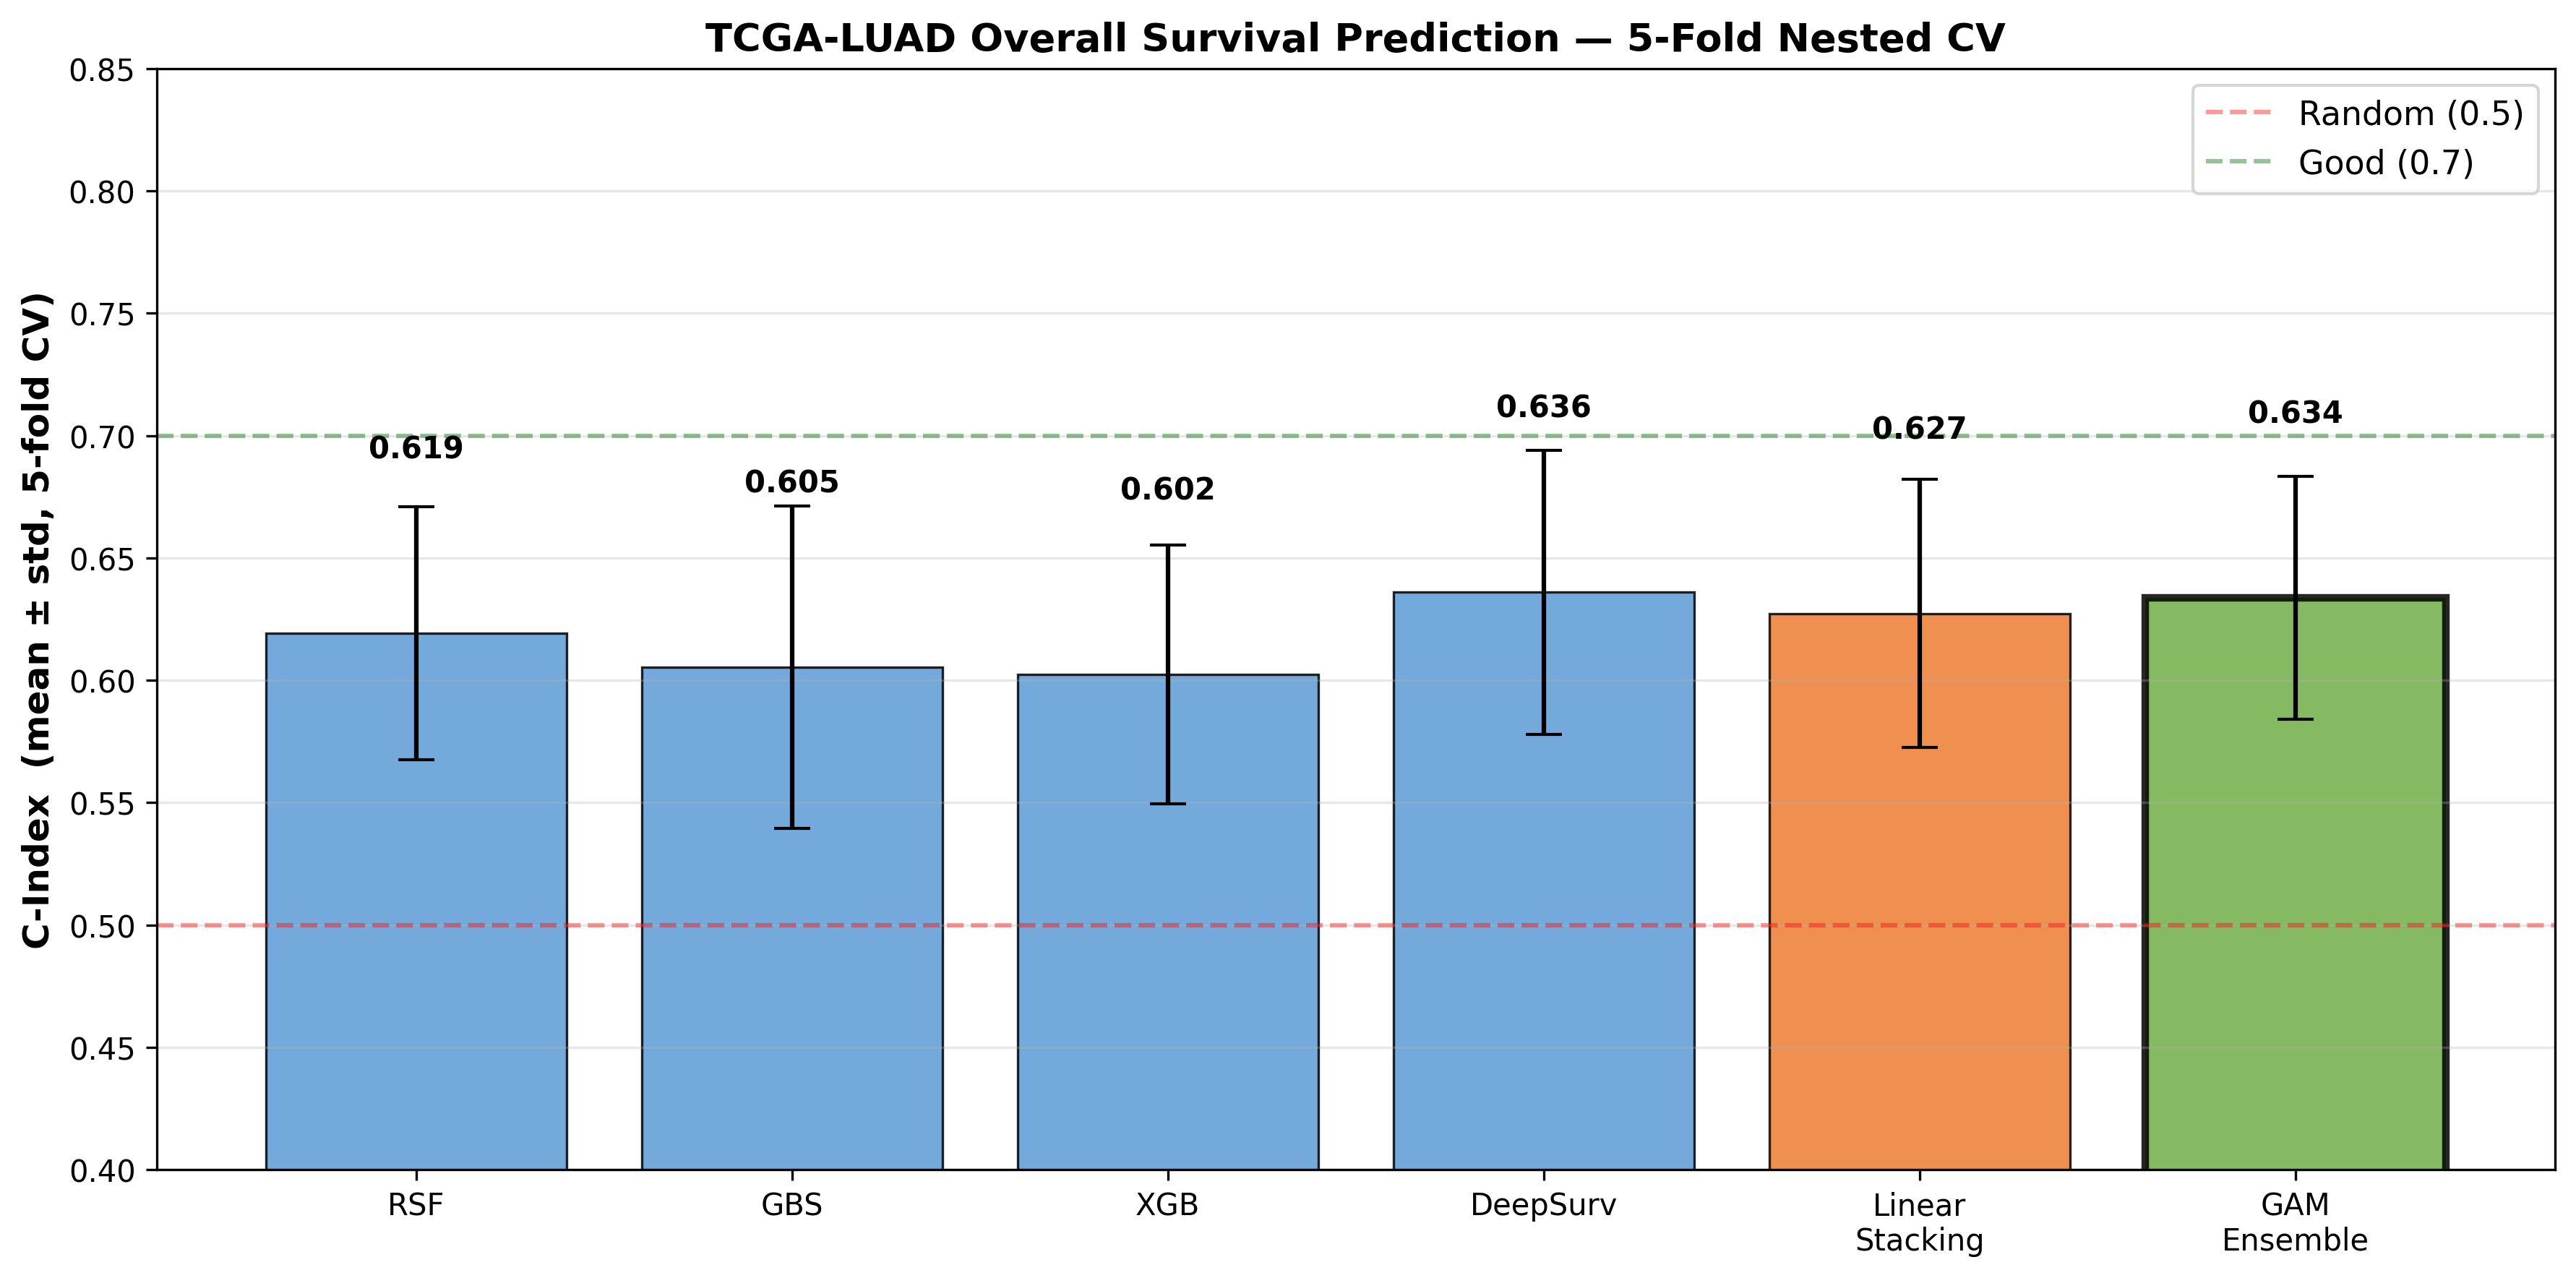
\includegraphics[width=\columnwidth]{performance_comparison.png}}
  \caption{Mean $\pm$ std C-index across five outer folds (TCGA-LUAD,
    5-fold nested CV). Stage-only Cox achieves the highest mean; SAGAM
    achieves the best stacking performance with lowest variance.}
  \label{fig:perf}
\end{figure}

\subsection{Per-Fold Analysis and Ablation}

Table~\ref{tab:results} provides fold-level C-indices.
SAGAM is the top-performing model in folds 1, 2, 4, and 5.
In fold~3, DeepSurv dominates (0.680) and SAGAM's advantage is reduced,
consistent with the observation that when a single base learner captures
nearly all available signal, ensemble integration provides limited benefit.
Wilcoxon signed-rank tests confirm directional but non-significant
SAGAM improvements: vs.\ Linear ($p\!=\!0.313$), vs.\ DeepSurv
($p\!=\!0.625$), vs.\ RSF ($p\!=\!0.094$).
With $n\!=\!5$ folds, the minimum achievable one-sided $p$ is 0.0625.
Bootstrap resampling (50,000 resamples) over folds shows 73.9\% of samples
favor SAGAM over linear stacking on C-index, and 93.8\% on IBS.
\textbf{With 181~OS events and $\approx$36 test events per fold, the study
is powered to detect C-index differences of $\approx$0.11; the observed
$\Delta\!=\!+0.006$ lies below this threshold, indicating that the observed
internal difference is too small to distinguish reliably from noise in the
current sample.}

Table~\ref{tab:ctdauc} reports time-dependent concordance AUC (Ctd-AUC),
a discrimination metric robust to censoring, computed at the 25th, 50th,
and 75th percentiles of training event times per fold, alongside Integrated
Brier Score (IBS), a time-dependent prediction-error metric requiring survival function estimates.
\textbf{SAGAM ties DeepSurv for the highest mean Ctd-AUC (0.650) and
achieves the best Ctd-AUC among stacking-based approaches}, with the lowest
fold-to-fold variance (std 0.054) among all stacking methods, mirroring
its C-index performance pattern and providing independent support that
SAGAM improves discrimination over linear stacking.
\textbf{SAGAM also achieves the lowest IBS (0.177\,$\pm$\,0.023), indicating
lower time-dependent prediction error compared to linear stacking
(0.184\,$\pm$\,0.030) and RSF (0.181\,$\pm$\,0.028).}
IBS was not reported for XGBoost-Cox and DeepSurv because the current
implementation did not estimate calibrated survival functions for these
models using a common baseline hazard procedure; future work will evaluate
survival-function calibration for all base learners under a unified
baseline hazard estimation framework.

\begin{table}[t]
\caption{Ctd-AUC (higher is better) and IBS (lower is better), mean\,$\pm$\,std
across 5 outer folds (TCGA-LUAD). IBS not reported for XGBoost-Cox and
DeepSurv (calibrated survival functions not estimated in current implementation).
SAGAM achieves the best value in both metrics among all stacking approaches.}
\label{tab:ctdauc}
\begin{center}
\setlength\tabcolsep{3pt}
\begin{tabular}{llcc}
\toprule
\textbf{Type} & \textbf{Model} & \textbf{Ctd-AUC} & \textbf{IBS} \\
\midrule
\multirow{4}{*}{Base} & RSF      & 0.634\,$\pm$\,0.068 & 0.181\,$\pm$\,0.028 \\
                      & GBS      & 0.614\,$\pm$\,0.069 & 0.197\,$\pm$\,0.042 \\
                      & XGBoost  & 0.626\,$\pm$\,0.067 & --- \\
                      & DeepSurv & 0.650\,$\pm$\,0.062 & --- \\
\midrule
\multirow{2}{*}{Stack}& Linear   & 0.642\,$\pm$\,0.066 & 0.184\,$\pm$\,0.030 \\
                      & \textbf{SAGAM} & \textbf{0.650\,$\pm$\,0.054} & \textbf{0.177\,$\pm$\,0.023} \\
\bottomrule
\end{tabular}
\end{center}
\end{table}

\begin{table}[t]
\caption{Per-Fold Test C-Indices (5-Fold Nested CV, TCGA-LUAD).
Among base learners and stacking methods, SAGAM is the top-performing
model in four of five folds. Stage-only Cox (not shown) is strongest
overall (0.657\,$\pm$\,0.044).}
\label{tab:results}
\begin{center}
\setlength\tabcolsep{3pt}
\begin{tabular}{ccccccc}
\toprule
\textbf{Fold} & \textbf{RSF} & \textbf{GBS} & \textbf{XGB}
              & \textbf{DS}  & \textbf{Linear} & \textbf{SAGAM} \\
\midrule
1 & 0.602 & 0.545 & 0.554 & 0.593 & 0.609 & \textbf{0.639} \\
2 & 0.584 & 0.584 & 0.620 & 0.592 & 0.584 & \textbf{0.604} \\
3 & 0.625 & 0.589 & 0.539 & \textbf{0.680} & 0.642 & 0.605 \\
4 & 0.706 & \textbf{0.718} & 0.646 & 0.716 & 0.716 & \textbf{0.718} \\
5 & 0.581 & 0.590 & 0.654 & 0.599 & 0.586 & \textbf{0.603} \\
\midrule
\textbf{Mean} & 0.619 & 0.605 & 0.602 & 0.636 & 0.627 & \textbf{0.634} \\
\bottomrule
\end{tabular}
\end{center}
\end{table}

\subsection{Spline Degree-of-Freedom Ablation}

Table~\ref{tab:df_ablation} shows SAGAM performance across spline complexity
settings, evaluated on the full four-learner ensemble by refitting only
the meta-learner with each df value using fixed OOF base learner predictions
from the main pipeline.
df\,=\,4 achieves the best mean C-index and lowest variance; higher df values
show increasing fold-to-fold variance consistent with overfitting when the
spline basis becomes too flexible relative to $\approx$145 training events.

\begin{table}[t]
\caption{Full 4-Learner SAGAM Spline df Sensitivity. Meta-learner refitted
across df values using \emph{fixed} OOF base learner predictions from the
main pipeline; these values are not directly comparable to Table~\ref{tab:baselines}
(0.634), which reruns the full nested training procedure per fold.
df\,=\,4 achieves the best mean C-index and lowest fold-to-fold variance
within this ablation.}
\label{tab:df_ablation}
\begin{center}
\begin{tabular}{lcc}
\toprule
\textbf{Variant} & \textbf{Mean C} & \textbf{Std} \\
\midrule
SAGAM df=3 & 0.610 & 0.061 \\
\textbf{SAGAM df=4} & \textbf{0.620} & \textbf{0.038} \\
SAGAM df=5 & 0.612 & 0.052 \\
SAGAM df=6 & 0.609 & 0.045 \\
\bottomrule
\end{tabular}
\end{center}
\end{table}

df\,=\,3 also underperforms, indicating insufficient flexibility to capture the
non-monotone smooth functions visible in Fig.~\ref{fig:smooths}.

\subsection{Clinical Risk Stratification}

Fig.~\ref{fig:km} shows Kaplan-Meier curves for pooled SAGAM OOF risk
tertiles across all 501 TCGA patients.
The low-risk group demonstrates markedly superior survival versus the
high-risk group (log-rank $p = 6.94 \times 10^{-5}$; multivariate
$p = 2.52 \times 10^{-4}$).
These pooled OOF predictions were never used during any training step,
confirming generalization to held-out patients.

\begin{figure*}[t]
  \centerline{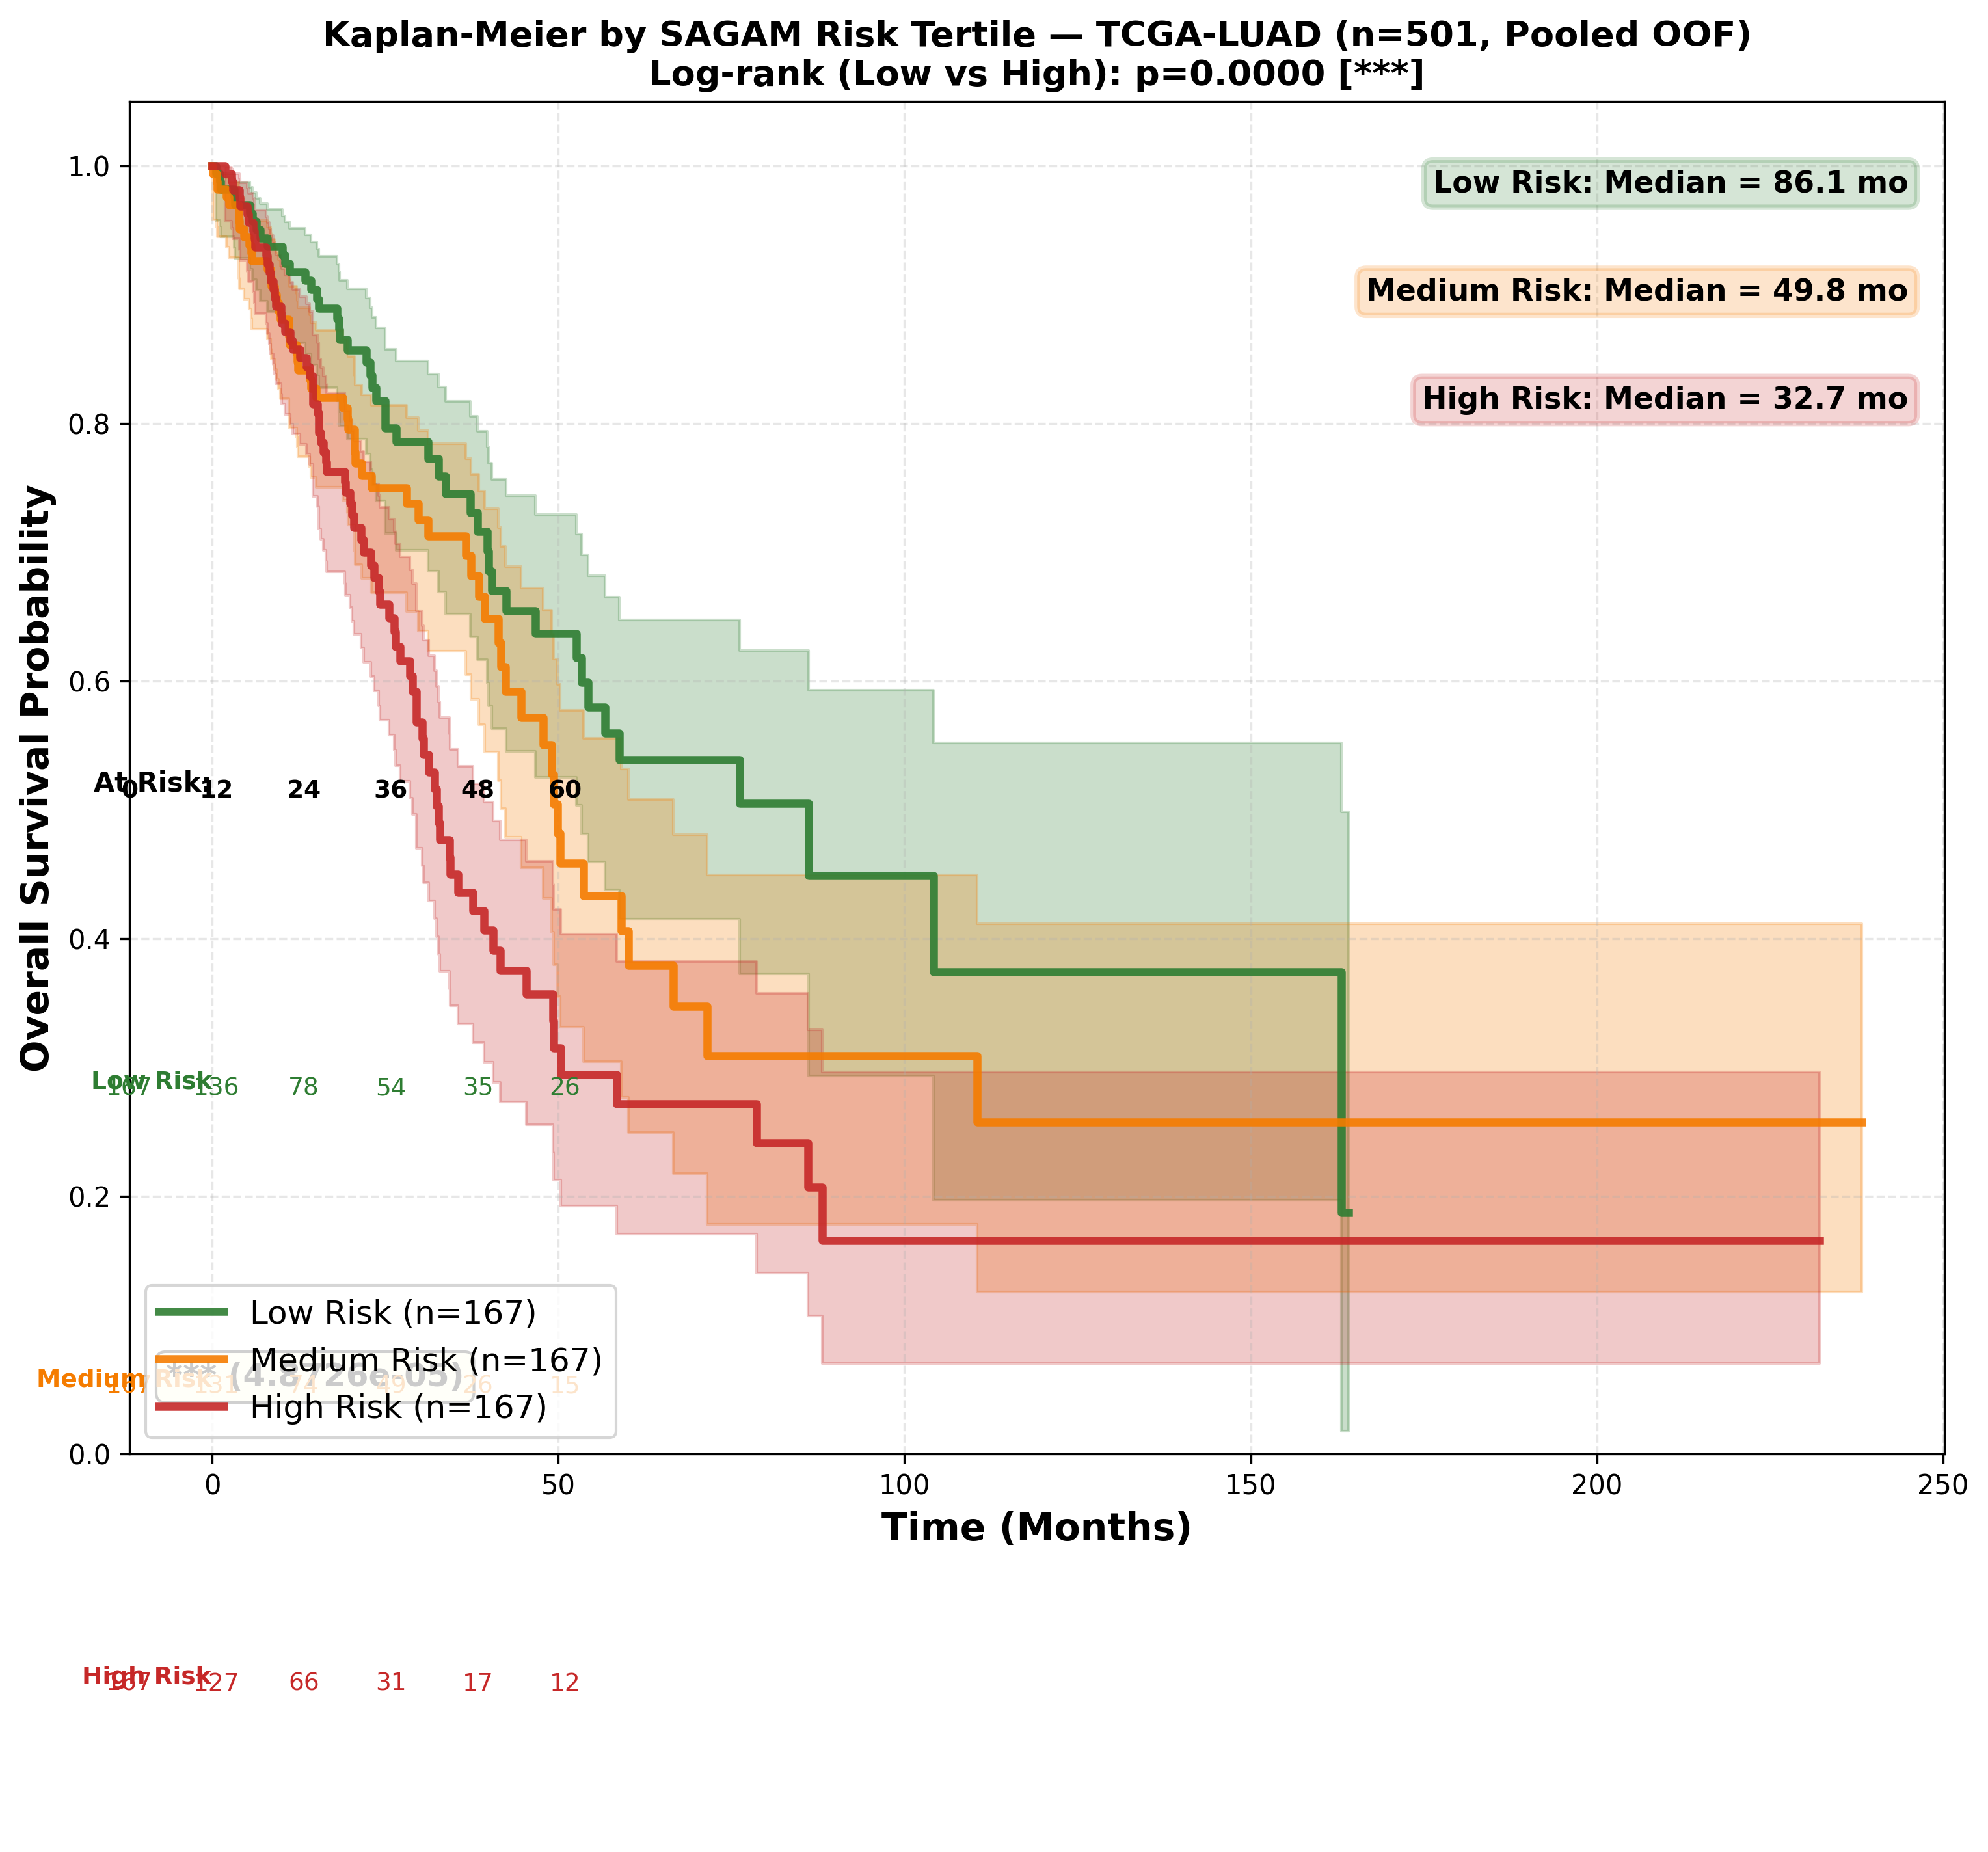
\includegraphics[width=0.78\textwidth]{kaplan_meier_nar.png}}
  \caption{Kaplan-Meier overall survival by SAGAM risk tertile with
    number-at-risk table. Pooled OOF predictions from 5-fold nested CV,
    TCGA-LUAD (n\,=\,501, 181 events).
    Log-rank (low vs.\ high): $p = 6.94\times10^{-5}$ (***).}
  \label{fig:km}
\end{figure*}

\subsection{Feature Block Analysis}

The Cox baseline results (Table~\ref{tab:baselines}) reveal a counterintuitive
pattern: adding features to a Cox model monotonically \emph{reduces}
discrimination.
Stage-only Cox (0.657) $>$ clinical-only (0.646) $>$ clinical+genomic
(0.641) $=$ all-features (0.641).
This consistent ordering suggests that added features do not improve the
penalized Cox baseline in this setting.

We attribute this pattern to two mechanisms.
First, \emph{feature collinearity}: several genomic and hypoxia features
are correlated with AJCC stage (e.g., aneuploidy increases with advancing
stage; hypoxia scores correlate with tumor size).
In a penalized linear model, collinear features dilute the stage coefficient
rather than providing additive predictive information.
Second, \emph{regularization masking}: CoxNet with an $\ell_1$ penalty
shrinks many added features to zero, yet even weak partial correlations
among retained features introduce estimation variance that outweighs their
marginal predictive contribution.

SAGAM's pipeline addresses a different problem by routing all features
through nonlinear base learners (RSF, GBS, XGBoost, DeepSurv) before
meta-learning.
Each base learner can identify nonlinear interactions between stage, genomic,
and hypoxia features that are invisible to a Cox model with linear main
effects.
The GAM meta-learner then integrates these nonlinear representations through
smooth functions.
This architecture explains why Table~\ref{tab:features} shows consistent
selection of Aneuploidy Score, Buffa Hypoxia, and TMB---features that add
no value to a linear Cox model.
Importantly, SAGAM does not exceed the strongest Cox baselines in internal
C-index; its contribution is instead improved nonlinear stacking over
scalar-weighted ensembles and interpretable model-level contribution
functions unavailable from any Cox model.

These results suggest that molecular and transcriptomic features may contain
nonlinear prognostic structure not captured by linear Cox models.
However, because SAGAM does not improve discrimination beyond AJCC stage,
this signal should be interpreted as useful for model-level analysis and
nonlinear ensemble behavior rather than demonstrated incremental clinical value.
SAGAM suggests that nonlinear base learners may extract structure from these
features, but the current results do not demonstrate incremental
discrimination beyond AJCC stage.

\subsection{Smooth Contribution Analysis}
\label{sec:nonlinear_analysis}

Fig.~\ref{fig:smooths} shows the smooth functions $f_k(s)$ from outer fold~1.
All four functions are nonlinear, validating the core SAGAM assumption
that scalar weights inadequately capture the meta-learning integration.

\begin{figure}[t]
  \centerline{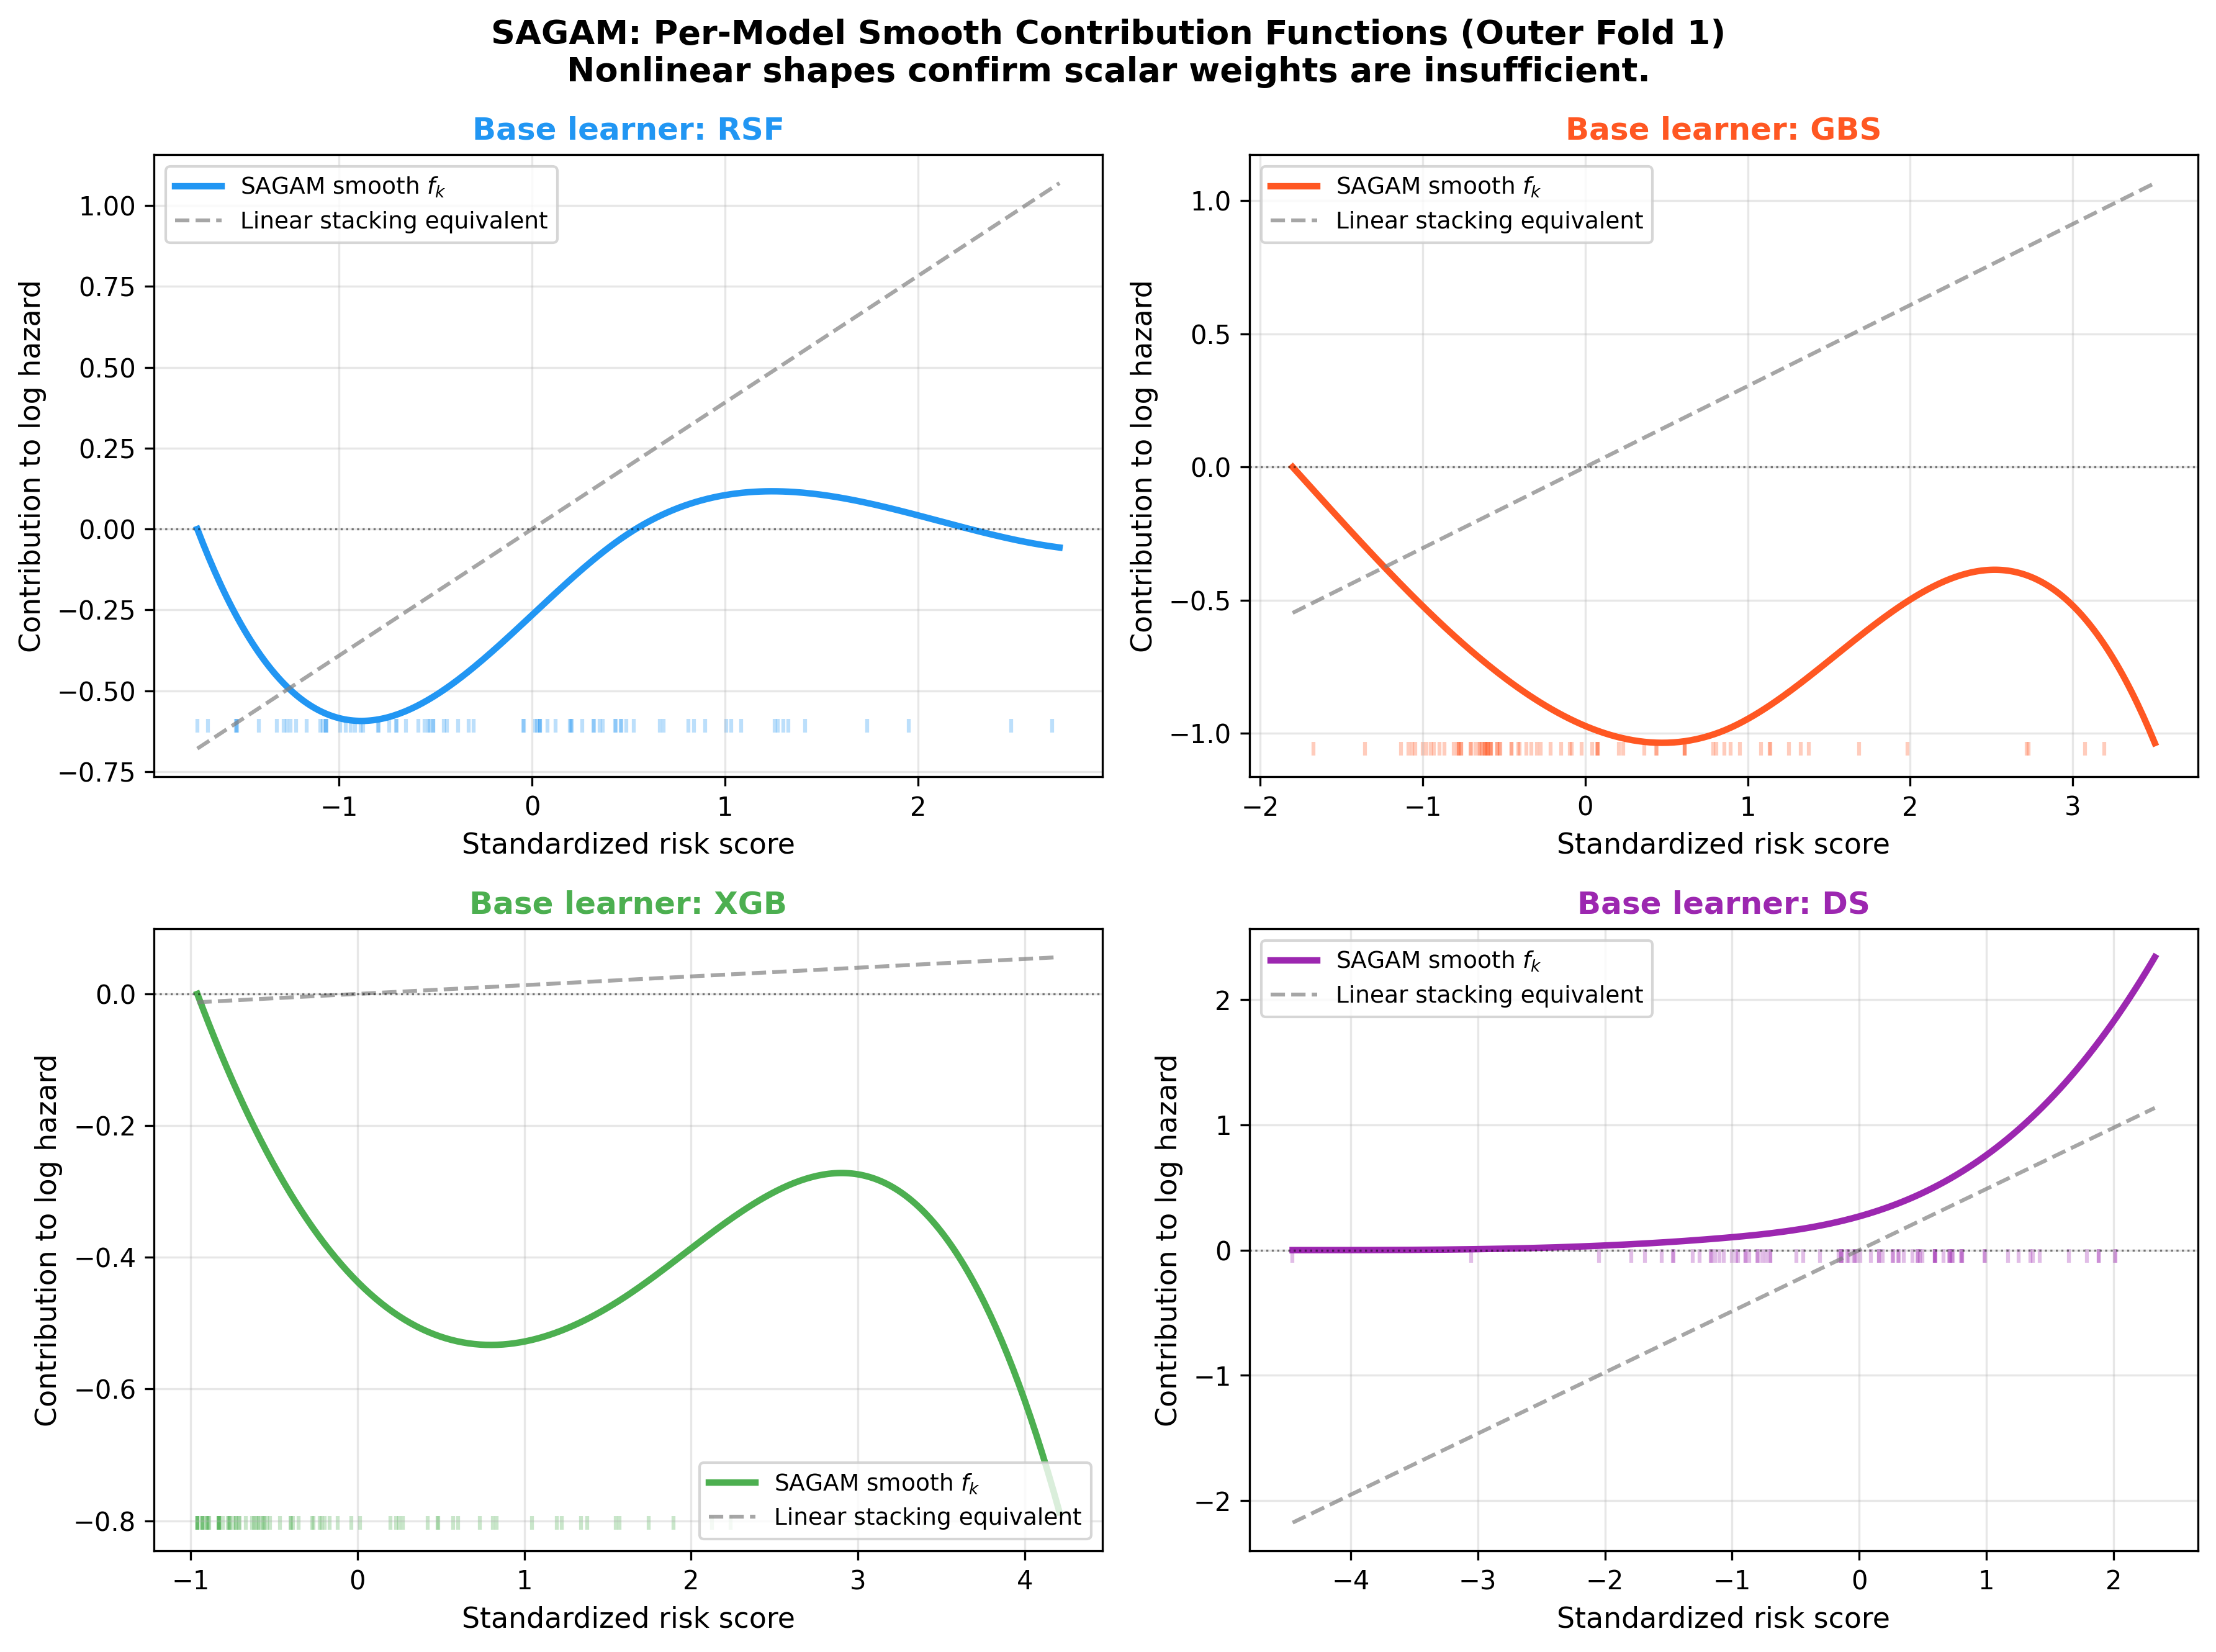
\includegraphics[width=\columnwidth]{gam_smooths_4panel.png}}
  \caption{SAGAM smooth contribution functions $f_k(s)$ per base learner
    (outer fold~1), each in its own panel. Standardized x-axis; dashed line
    shows linear stacking equivalent. All four functions are nonlinear,
    validating the B-spline parameterization.}
  \label{fig:smooths}
\end{figure}

DeepSurv and RSF exhibit the steepest gradients, consistent with their
highest individual C-indices.
GBS and XGBoost show flatter curves, indicating partial redundancy
with stronger learners.
The non-monotone shape for DeepSurv---saturating at high risk scores---is
a score-range-dependent pattern that a fixed positive scalar weight cannot
express, justifying the B-spline parameterization.

\subsection{Nonlinearity Quantification}
\label{sec:nonlinear_quant}

Table~\ref{tab:nonlinearity} quantifies the nonlinearity of each smooth
function $f_k$ across all five outer folds.
For each fold, we evaluate $f_k(s)$ on a 300-point grid, fit a linear
regression to $(s, f_k(s))$, and compute (i) the nonlinearity fraction
$1 - R^2_{\text{linear}}$ (fraction of $f_k$ variance not explained by a
linear fit) and (ii) the root mean squared deviation (RMSD) from the
linear fit.

\begin{table}[t]
\caption{Nonlinearity of SAGAM Smooth Functions $f_k$ (Mean Across 5 Folds).
NonlinFrac = $1 - R^2_{\text{linear}}$; RMSD = deviation from best-fit line.
All four base learners show substantial nonlinearity, confirming that a
fixed scalar weight cannot adequately represent their contribution.}
\label{tab:nonlinearity}
\begin{center}
\begin{tabular}{lcc}
\toprule
\textbf{Base Learner} & \textbf{NonlinFrac} & \textbf{RMSD} \\
\midrule
RSF      & 0.349 & 0.208 \\
GBS      & 0.402 & 0.153 \\
XGBoost  & 0.337 & 0.254 \\
DeepSurv & 0.424 & 0.276 \\
\bottomrule
\end{tabular}
\end{center}
\end{table}

All four base learners exhibit substantial nonlinearity (NonlinFrac $> 0$),
with DeepSurv showing the largest deviation consistent with its non-monotone
curve in Fig.~\ref{fig:smooths}.
These results confirm that a fixed scalar weight $\gamma_k$---equivalent to
a linear function $f_k(s) = \gamma_k s$---inadequately represents
the base learner's contribution across the full risk spectrum.

Fig.~\ref{fig:stability} shows the smooth functions $f_k$ across all five
outer folds.
The nonlinear shapes are consistent across folds for all four base learners,
confirming that the observed nonlinearity reflects stable structure in the
data rather than fold-specific artifacts.

\begin{figure}[t]
  \centerline{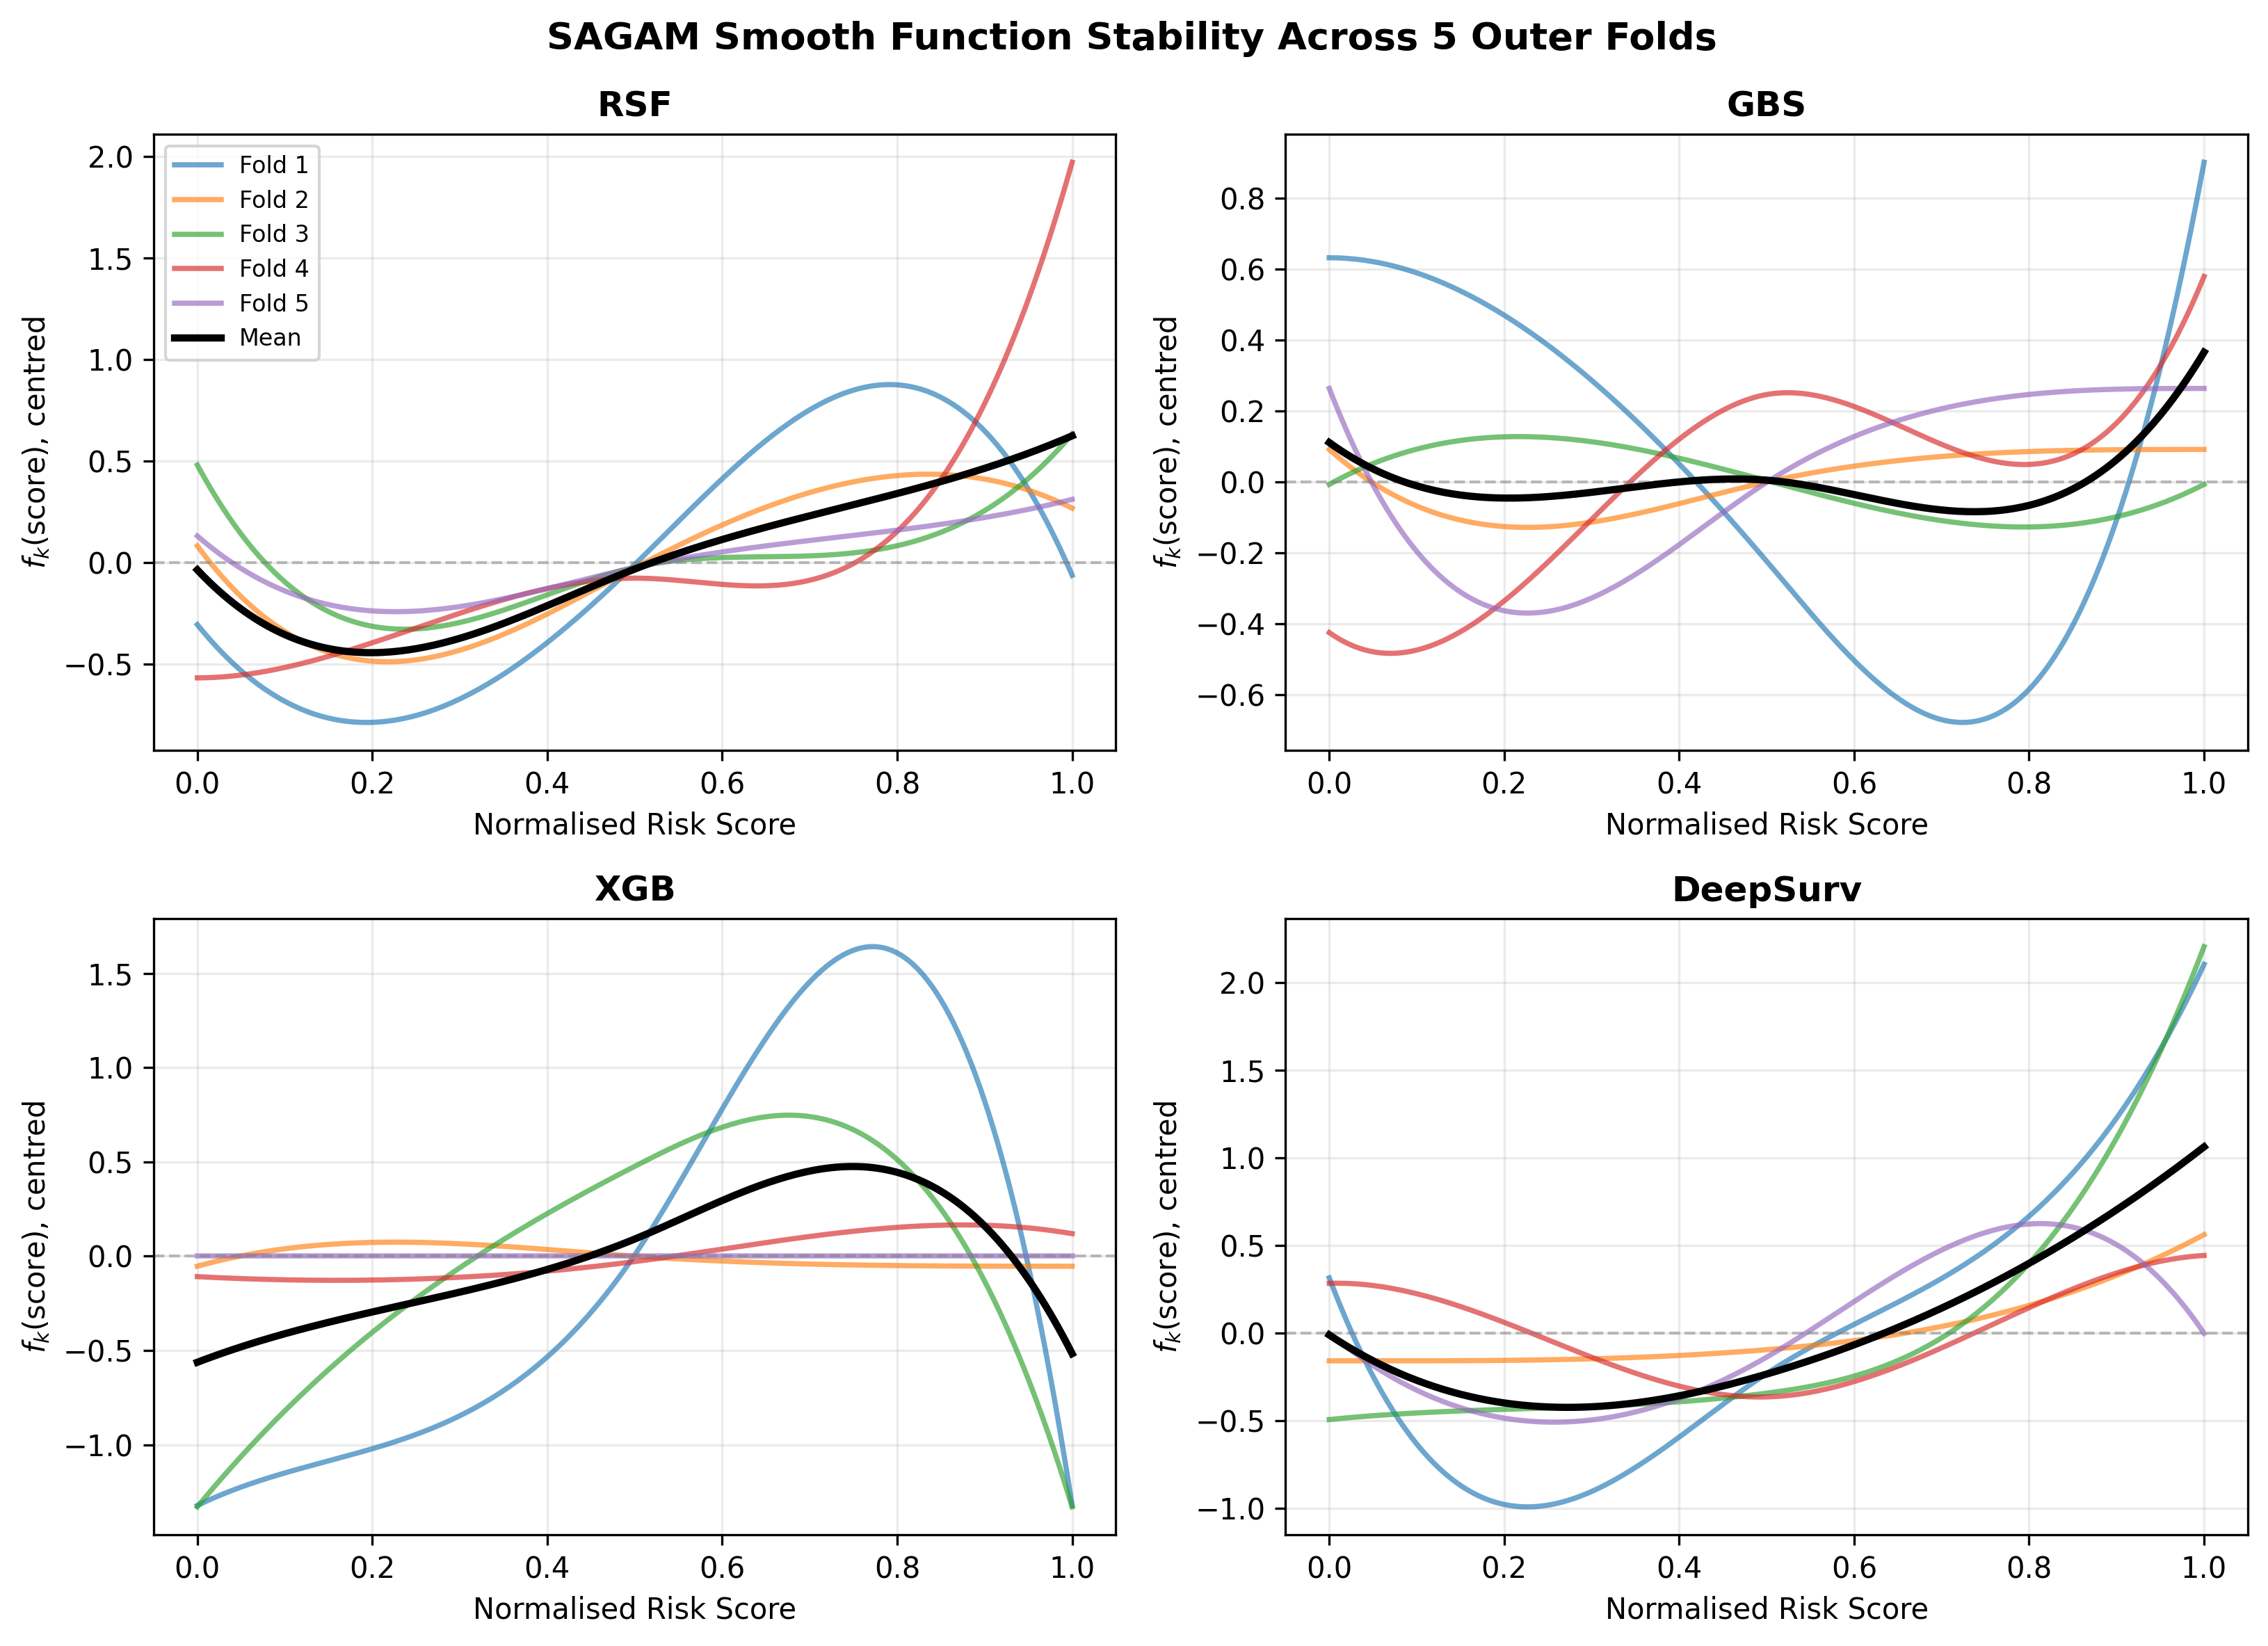
\includegraphics[width=\columnwidth]{gam_smooths_stability.png}}
  \caption{SAGAM smooth function $f_k$ stability across all 5 outer folds.
    Each panel shows one base learner; thin lines = individual folds;
    thick black line = mean. The consistent nonlinear shapes across folds
    confirm that the nonlinearity is a stable data property, not a
    fold-specific artifact.}
  \label{fig:stability}
\end{figure}

Fig.~\ref{fig:brier} shows the time-dependent Brier score (outer fold~1),
confirming that SAGAM's lower time-dependent prediction error over linear
stacking and RSF is consistent across the follow-up horizon.

\begin{figure}[t]
  \centerline{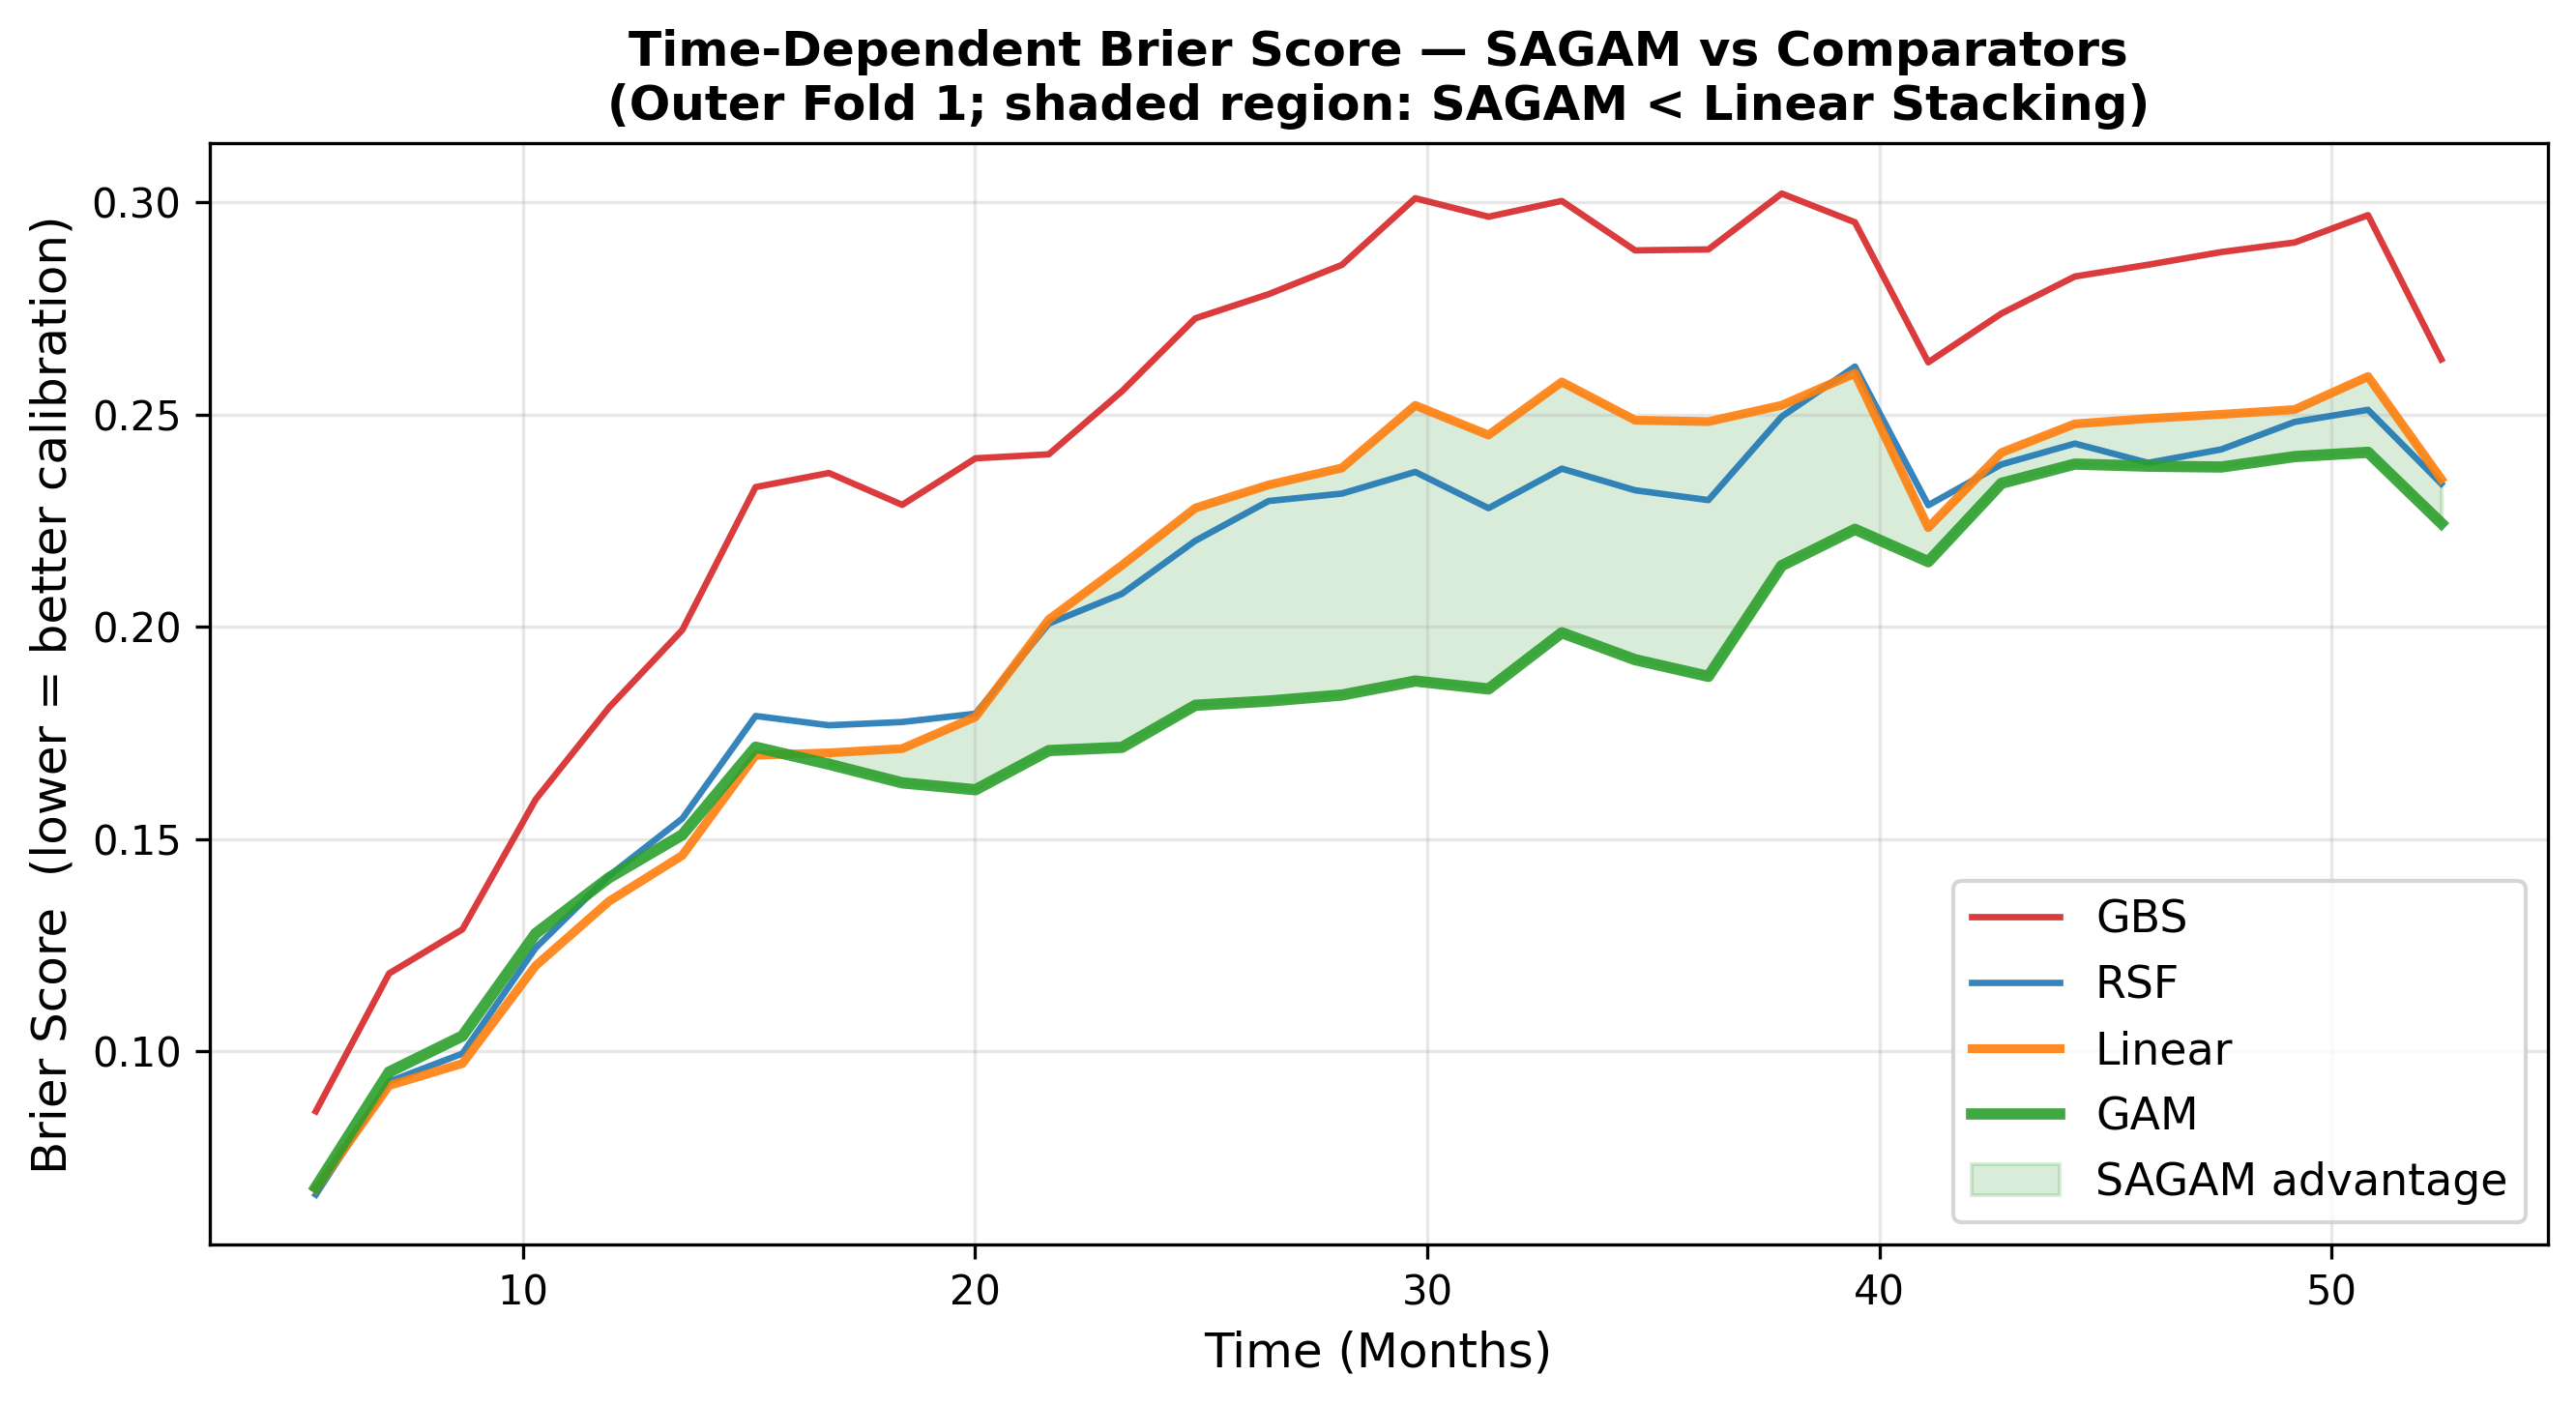
\includegraphics[width=\columnwidth]{brier_score_time.png}}
  \caption{Time-dependent Brier score (outer fold~1; lower = lower
    time-dependent prediction error). Shaded region: time points where
    SAGAM $<$ Linear Stacking. Mean IBS across all 5 folds: SAGAM 0.177,
    Linear 0.184, RSF 0.181, GBS 0.197 (Table~\ref{tab:ctdauc}).}
  \label{fig:brier}
\end{figure}

\subsection{Subgroup Analysis by AJCC Stage}
\label{sec:subgroup}

Table~\ref{tab:subgroup} reports pooled OOF C-indices stratified by
AJCC pathological stage using all 501 TCGA patients.
SAGAM's advantage over linear stacking is largest in Stage~I/II patients
($\Delta\!=\!+0.010$, n\,=\,394, 120 events), where molecular and genomic
features may contribute to heterogeneous base learner behavior, and
smaller in Stage~III/IV ($\Delta\!=\!+0.005$, n\,=\,105, 61 events), where
advanced-stage clinical signals dominate and linear combination already
captures most available information.
This stage-dependent pattern is consistent with the GSE31210 (stage~I/II only)
external result ($\Delta\!=\!+0.086$) and the GSE68465 (all stages)
result ($\Delta\!=\!-0.026$): SAGAM's nonlinear integration provides the
most benefit when base learner performance is heterogeneous.

\begin{table}[t]
\caption{Subgroup Analysis by AJCC Stage (Pooled OOF, 501 TCGA patients).
SAGAM's advantage is largest in Stage~I/II, where SAGAM shows its largest
observed advantage over linear stacking.}
\label{tab:subgroup}
\begin{center}
\begin{tabular}{lcccc}
\toprule
\textbf{Group} & \textbf{n} & \textbf{Events} & \textbf{C(GAM)} & \textbf{C(Lin)} \\
\midrule
Stage I/II  & 394 & 120 & 0.574 & 0.564 \\
Stage III/IV & 105 &  61 & 0.582 & 0.577 \\
All patients & 501 & 181 & 0.625 & 0.619 \\
\bottomrule
\end{tabular}
\end{center}
\end{table}

\subsection{Feature Selection Stability}

Table~\ref{tab:features} reports the ten most stably selected features.
AJCC stage, Aneuploidy Score, and Buffa Hypoxia Score are selected in all
five folds.
Interestingly, the Cox baseline analysis (Table~\ref{tab:baselines}) shows
that adding genomic and hypoxia features to a Cox model does not improve over
stage-only Cox, yet these features are consistently selected as part of the
full SAGAM feature matrix.
This suggests that RSF, GBS, XGBoost, and DeepSurv can extract nonlinear
interactions among these features that the linear Cox model cannot, and
SAGAM's smooth meta-learning then integrates those signals.

\begin{table}[t]
\caption{Top-10 Stably Selected Features (5-Fold Nested CV)}
\label{tab:features}
\begin{center}
\begin{tabular}{lcc}
\toprule
\textbf{Feature} & \textbf{Folds} & \textbf{Category} \\
\midrule
AJCC Pathologic Tumor Stage    & 5/5 & Clinical \\
Aneuploidy Score               & 5/5 & Genomic \\
Buffa Hypoxia Score            & 5/5 & Hypoxia \\
Age at Diagnosis               & 5/5 & Clinical \\
TMB (nonsynonymous)            & 4/5 & Genomic \\
MSI MANTIS Score               & 4/5 & Genomic \\
Ragnum Hypoxia Score           & 4/5 & Hypoxia \\
Path T Stage                   & 4/5 & Clinical \\
Tumor Break Load               & 3/5 & Genomic \\
Path N Stage                   & 3/5 & Clinical \\
\bottomrule
\end{tabular}
\end{center}
\end{table}

\subsection{External Validation on Two Independent Cohorts}

Table~\ref{tab:external} reports concordance indices on two independent
GEO cohorts, with SAGAM trained exclusively on TCGA.
GSE31210 (Takeuchi et al., 226 stage~I/II pure LUAD, 35 OS events) and
GSE68465 (Director's Challenge Consortium, 432 mixed-stage LUAD, 226 OS events)
represent qualitatively different external test settings.

\begin{table}[t]
\caption{External Validation on Two Independent LUAD Cohorts.
SAGAM outperforms linear stacking on stage~I/II LUAD
(GSE31210, $\Delta\!=\!+0.086$) but not on the all-stage Director's
Challenge cohort (GSE68465, $\Delta\!=\!-0.026$), consistent with
stage-dependent subgroup patterns observed internally.
$^\dagger$KM log-rank $p$ tests SAGAM risk-group separation, not
C-index superiority over linear stacking.
Bootstrap CIs reported for stacking models; base-learner CIs were omitted
to focus uncertainty reporting on the primary stacking comparison (future
work will report uncertainty for all external models).
Stage-only Cox not evaluated on GSE68465 (stage not sufficiently harmonized).}
\label{tab:external}
\begin{center}
\setlength\tabcolsep{2pt}
\begin{tabular}{lcccc}
\toprule
& \multicolumn{2}{c}{\textbf{GSE31210}} & \multicolumn{2}{c}{\textbf{GSE68465}} \\
& \multicolumn{2}{c}{\scriptsize Stage~I/II, $n\!=\!226$, 35 ev.} &
  \multicolumn{2}{c}{\scriptsize All stages, $n\!=\!432$, 226 ev.} \\
\cmidrule(lr){2-3}\cmidrule(lr){4-5}
\textbf{Model} & \textbf{C} & \textbf{CI} & \textbf{C} & \textbf{CI} \\
\midrule
Stage-only Cox   & \textbf{0.678} & --- & \multicolumn{2}{c}{\scriptsize stage not harmonized} \\
\midrule
RSF              & 0.541 & --- & 0.576 & --- \\
GBS              & 0.477 & --- & 0.554 & --- \\
XGBoost-Cox      & 0.538 & --- & 0.548 & --- \\
DeepSurv         & 0.626 & --- & 0.572 & --- \\
\midrule
Linear Stacking  & 0.510 & {\scriptsize[0.390, 0.616]} & 0.575 & {\scriptsize[0.533, 0.612]} \\
\textbf{SAGAM}   & \textbf{0.596} & \textbf{\scriptsize[0.483, 0.709]} & 0.549 & {\scriptsize[0.508, 0.589]} \\
\midrule
$\Delta$ C-index       & \multicolumn{2}{c}{$\mathbf{+0.086}$}
                       & \multicolumn{2}{c}{$-0.026$} \\
KM log-rank $p^\dagger$ & \multicolumn{2}{c}{$0.030$}
                       & \multicolumn{2}{c}{$0.153$} \\
\bottomrule
\end{tabular}
\end{center}
\end{table}

On GSE31210, SAGAM (0.596) outperforms linear stacking by $+0.086$---a
larger observed advantage than the internal $+0.006$---with significant risk
stratification ($p\!=\!0.030$; Fig.~\ref{fig:ext_km}).
On GSE68465, SAGAM (0.549) does not outperform linear stacking (0.575,
$\Delta\!=\!-0.026$, NS).
This cohort-level divergence is clinically interpretable: in GSE68465,
all four base learners perform similarly (RSF 0.576, DS 0.572, GBS 0.554,
XGB 0.548), leaving little room for score-range-dependent reweighting;
in GSE31210, DeepSurv (0.626) dominates other base learners (GBS 0.477),
and SAGAM's smooth functions can effectively up-weight the dominant learner
while down-weighting the weaker ones.
This pattern is also consistent with the internal subgroup analysis
(Section~\ref{sec:subgroup}): SAGAM's advantage is largest in Stage~I/II
($\Delta\!=\!+0.010$, where base learner performance is most heterogeneous)
compared to Stage~III/IV ($\Delta\!=\!+0.005$).

\begin{figure*}[t]
  \centerline{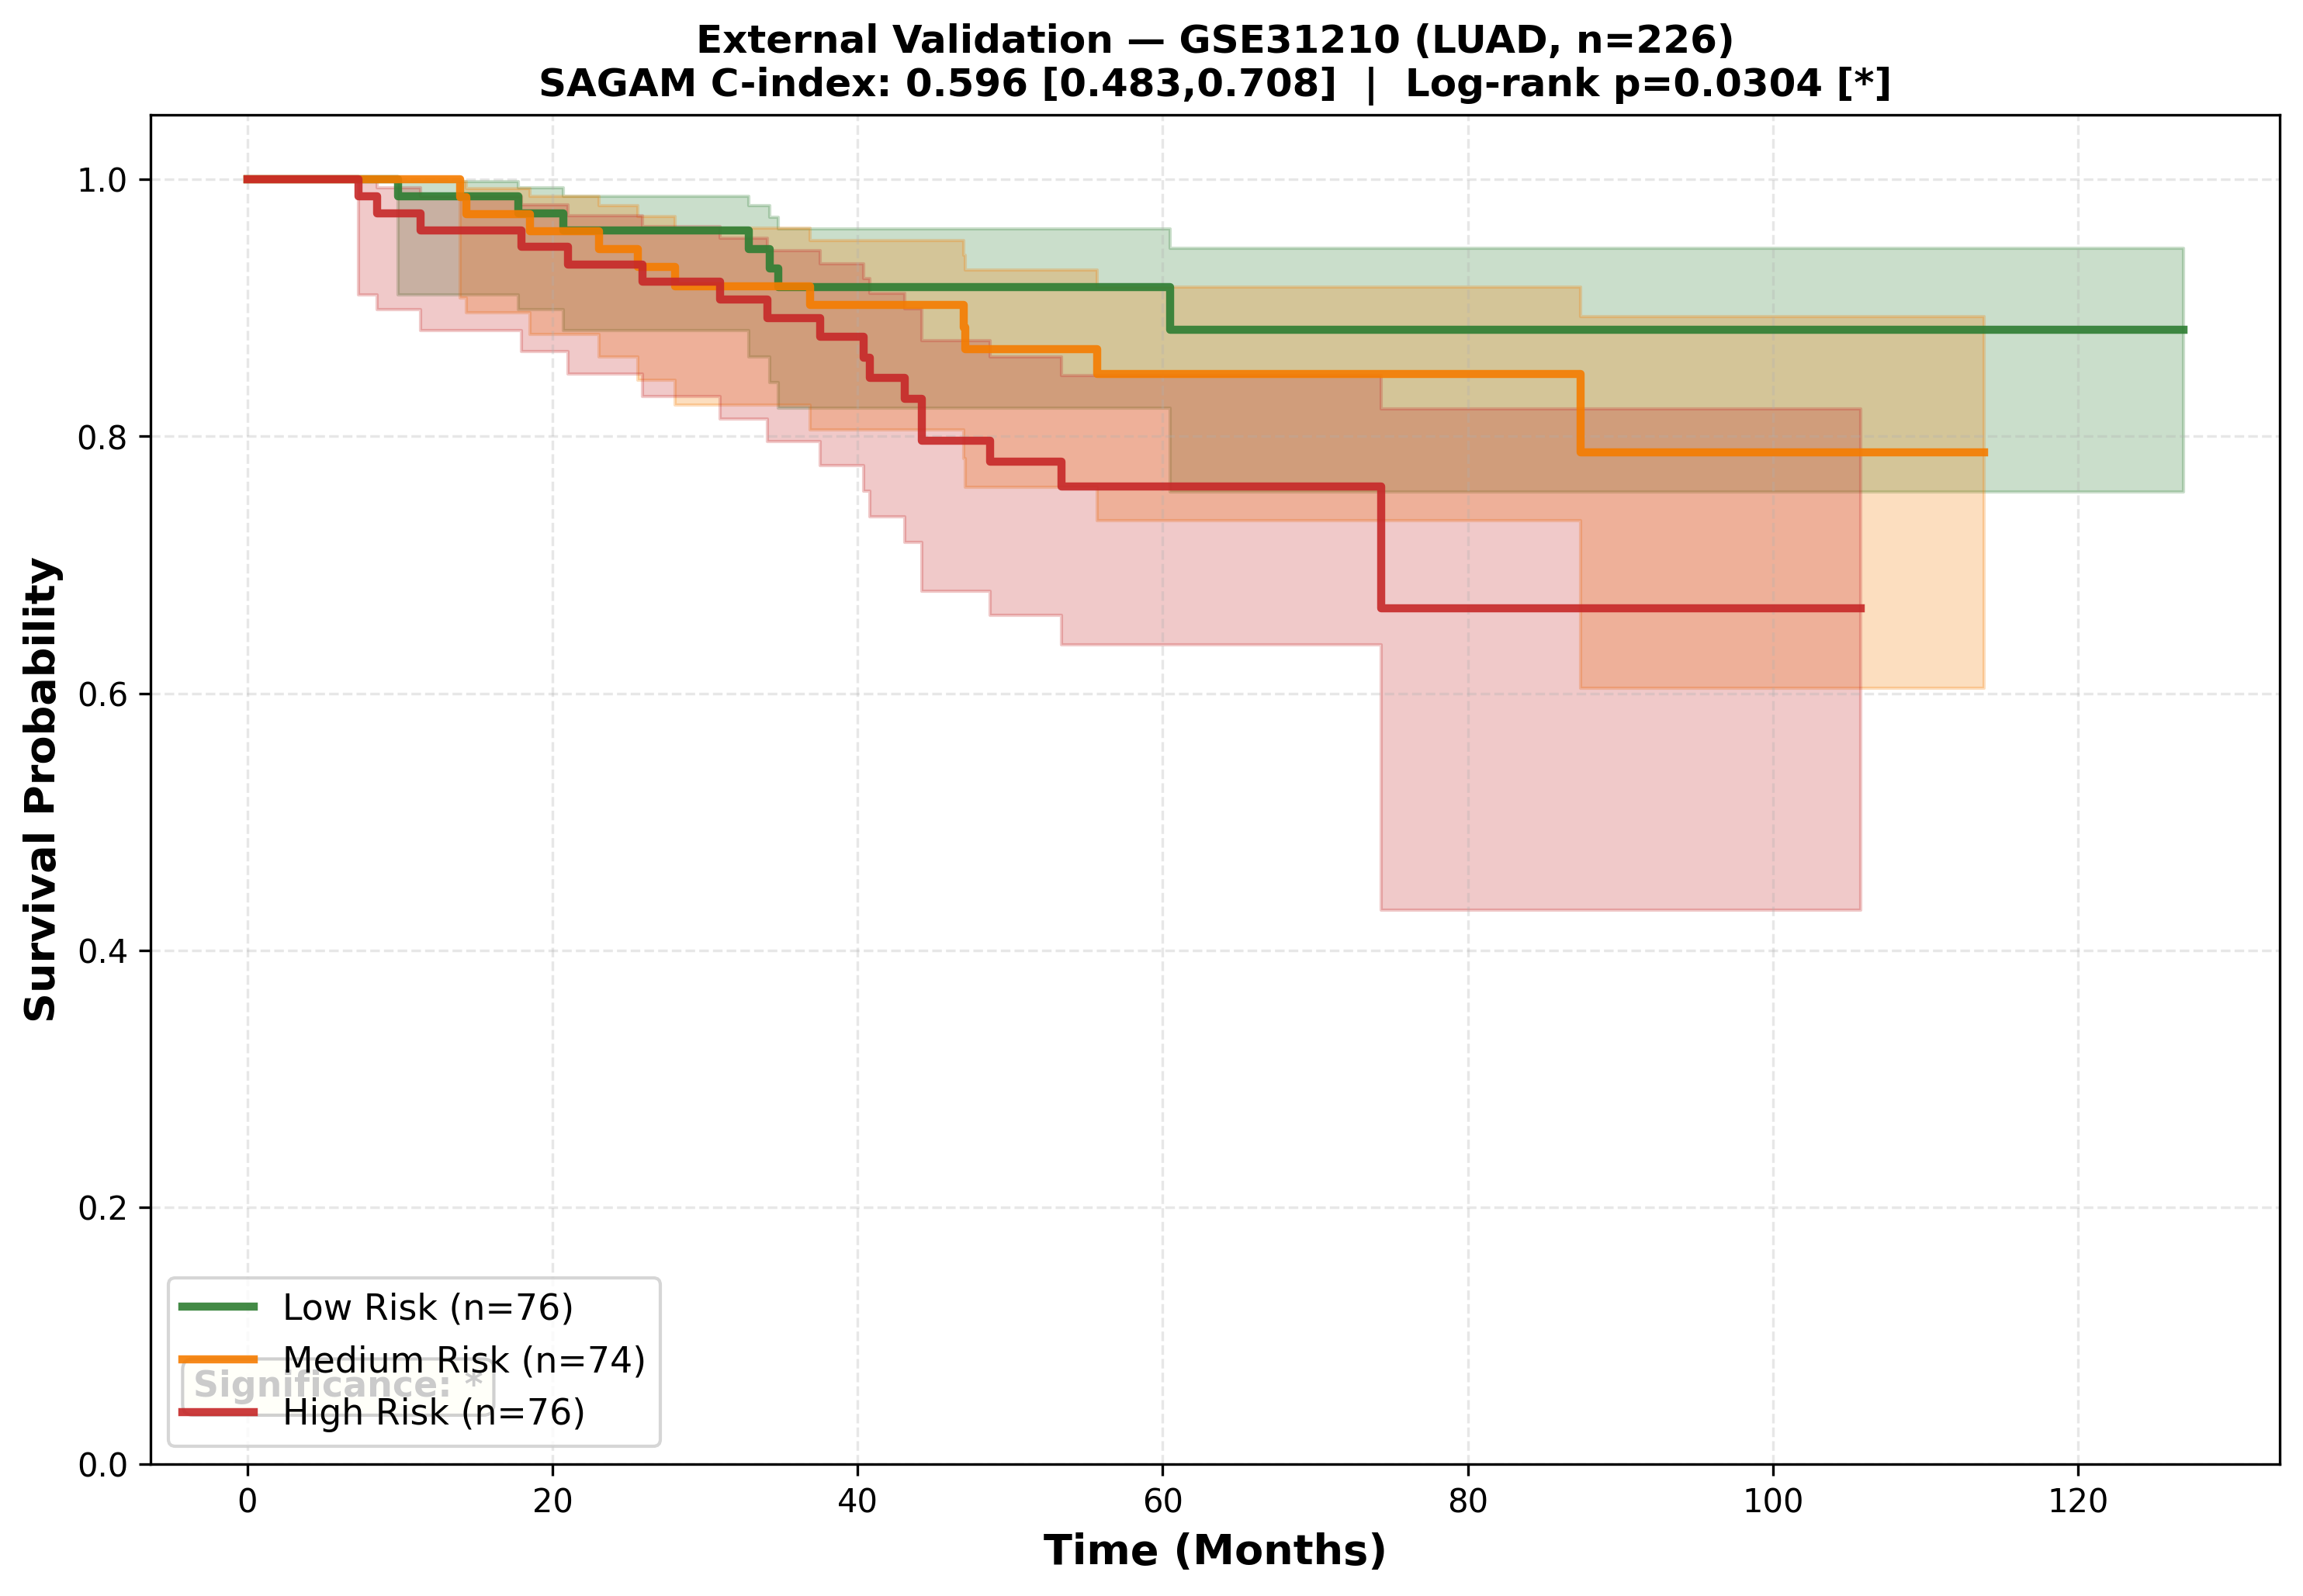
\includegraphics[width=0.78\textwidth]{ext_kaplan_meier.png}}
  \caption{External validation Kaplan-Meier curves on GSE31210
    (n\,=\,226, stage I/II pure LUAD, 35 OS events).
    SAGAM trained on TCGA only.
    Log-rank (low vs.\ high): $p = 0.030$ (*).}
  \label{fig:ext_km}
\end{figure*}

\begin{figure*}[t]
  \centerline{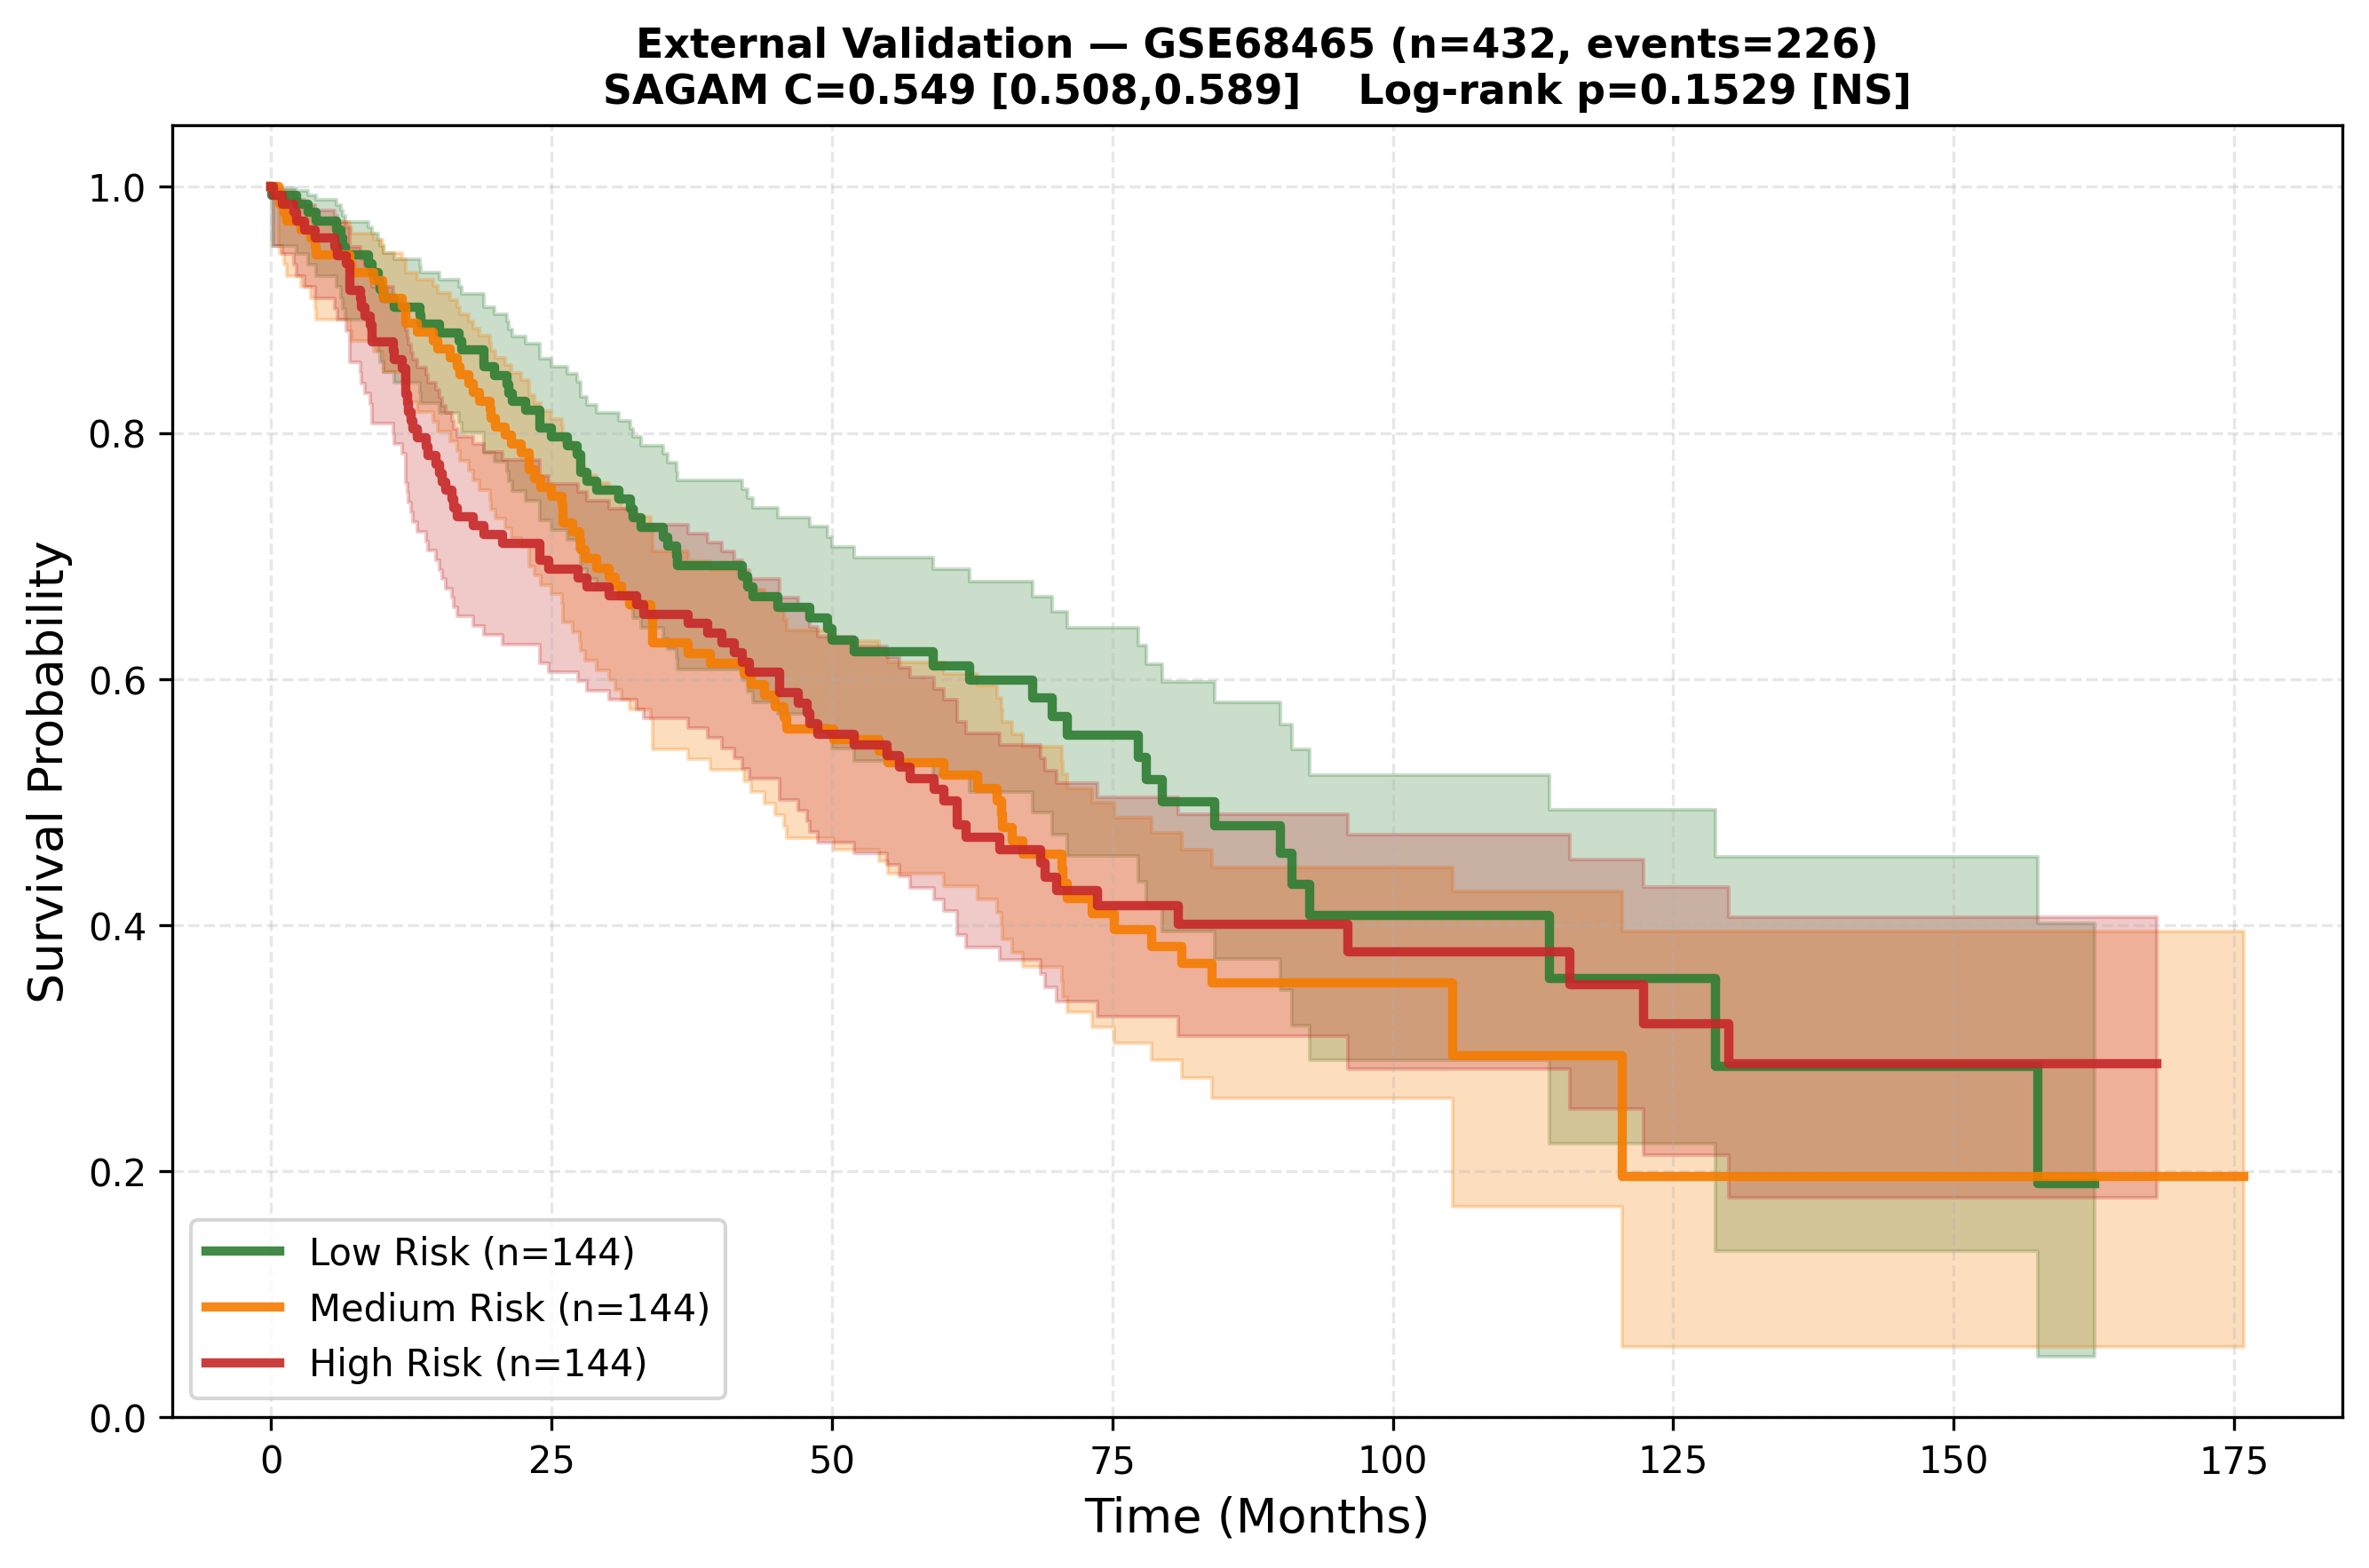
\includegraphics[width=0.78\textwidth]{ext_km_gse68465.png}}
  \caption{External validation Kaplan-Meier curves on GSE68465 (Director's
    Challenge Consortium; n\,=\,432, all stages, 226 OS events).
    SAGAM trained on TCGA only ($\Delta$(SAGAM$-$Linear)\,=\,$-0.026$, NS).
    Unlike the stage~I/II GSE31210 cohort, base learners perform within a
    narrow band (0.548--0.576), leaving little room for nonlinear reweighting.}
  \label{fig:ext_km_gse68465}
\end{figure*}

% ============================================================
\section{Discussion}
% ============================================================

\textbf{AJCC stage is the strongest predictor, internally and externally.}
Stage-only Cox dominates all models in both evaluations: 0.657 internally
and 0.678 externally on GSE31210, exceeding DeepSurv (0.626) and SAGAM
(0.596) on the external cohort.
Combining SAGAM risk scores with stage (Stage~+~SAGAM = 0.653) does not
improve over stage alone (0.657), confirming that SAGAM's learned risk
scores do not carry substantial incremental prognostic information beyond
AJCC staging.
These findings reinforce that \emph{SAGAM's contribution is methodological},
not clinical superiority: it provides an interpretable nonlinear stacking
mechanism that improves over linear stacking and exposes per-model
contribution functions, but should not be presented as a replacement for
AJCC staging in clinical decision-making.

\textbf{What SAGAM adds over linear stacking.}
All prior survival stacking
methods~\cite{lyu2026supersurv,golmakani2024joint,zhao2024bayesian,
vock2016adapting,huang2023twostage} assign fixed scalar weights to base
learner predictions.
SAGAM replaces scalar weights with smooth B-spline functions, allowing
the meta-learner to capture score-range-dependent integration
rules~\eqref{eq:sagam}.
\textbf{The strongest supportive evidence comes from GSE31210, where SAGAM
outperforms linear stacking by $+0.086$, compared with $+0.006$ internally;
GSE68465 shows this benefit depends on cohort structure and base-learner
heterogeneity.}
When base-learner score distributions shift between training and test cohorts,
linear stacking's fixed scalar weights may become miscalibrated across the
full risk spectrum.
SAGAM's smooth functions may adapt the integration rule to different score
ranges, but the mixed external results indicate that this benefit depends
on cohort composition and base-learner heterogeneity.
SAGAM also achieves the lowest Integrated Brier Score (IBS\,=\,0.177)
among all models with comparable IBS support, indicating lower
time-dependent prediction error compared to linear stacking (0.184)
and RSF (0.181), providing further support that SAGAM's integration
reduces prediction error beyond C-index alone.
The smooth functions (Fig.~\ref{fig:smooths}) confirm that all four base
learners exhibit nonlinear relationships to the ensemble log-hazard,
providing qualitative validation of the B-spline parameterization (see also
Section~\ref{sec:nonlinear_analysis} for quantitative nonlinearity analysis).

\textbf{DeepSurv as the strongest base learner.}
DeepSurv achieves the highest raw C-index externally (0.626) and ties SAGAM
internally (0.636 vs.\ 0.634).
Table~\ref{tab:deepsurv_compare} contrasts SAGAM and DeepSurv along
multiple dimensions.
SAGAM's primary value is not raw C-index superiority but interpretable
nonlinear ensemble integration: its smooth contribution functions reveal
where in the risk spectrum each model contributes, information unavailable
from a neural black-box.

\begin{table}[t]
\caption{DeepSurv vs.\ SAGAM: Complementary Roles}
\label{tab:deepsurv_compare}
\begin{center}
\setlength\tabcolsep{3pt}
\begin{tabular}{lcc}
\toprule
\textbf{Criterion} & \textbf{DeepSurv} & \textbf{SAGAM} \\
\midrule
Internal mean C-index      & 0.636 & 0.634 \\
GSE31210 C-index           & \textbf{0.626} & 0.596 \\
GSE68465 C-index           & 0.572 & 0.549 \\
Fold-to-fold std           & 0.058 & \textbf{0.050} \\
Ensemble integration       & no    & yes (4 learners) \\
Interpretable contribution & no    & smooth $f_k$ \\
Advantage over linear stk  & n/a   & +0.006 (int); +0.086 (GSE31210) \\
\bottomrule
\end{tabular}
\end{center}
\end{table}

\textbf{Stage-dependent external advantage.}
External validation on two independent cohorts reveals a nuanced picture.
On GSE31210 (stage~I/II, 35 events), SAGAM outperforms linear stacking by
$+0.086$---a larger observed advantage than the internal $+0.006$.
On GSE68465 (Director's Challenge, all stages, 226 events), SAGAM does
\emph{not} outperform linear stacking ($\Delta\!=\!-0.026$, NS).
This divergence aligns with the internal subgroup analysis: SAGAM's
advantage is $+0.010$ in Stage~I/II (where base learner performance is most
heterogeneous) versus $+0.005$ in Stage~III/IV (where clinical stage
dominates and linear combination already captures most available information).
The mechanism is further supported by base learner heterogeneity:
on GSE31210, DeepSurv (0.626) substantially outperforms GBS (0.477),
creating a heterogeneous performance landscape that SAGAM's smooth
functions can exploit; on GSE68465, all learners perform within a
narrow band (0.548--0.576), leaving little gain for nonlinear reweighting.
These results establish a clearer scope for SAGAM: \emph{its nonlinear
integration is most beneficial when base learners have heterogeneous
performance profiles.}

\textbf{Feature interactions and nonlinear signal.}
A key finding from Table~\ref{tab:baselines} is that linear Cox models fail
to benefit from molecular features (genomic, hypoxia) beyond what stage
alone provides.
Yet Table~\ref{tab:features} shows these same features are stably selected
across SAGAM's folds.
This apparent contradiction resolves when one recognizes that RSF and GBS
can extract nonlinear interactions among stage, Aneuploidy Score, hypoxia
scores, and TMB that are invisible to a linear model.
SAGAM's smooth meta-learning then integrates these nonlinearly-extracted
signals, explaining why it substantially outperforms linear stacking even
with a modest internal C-index gain.

\textbf{Scalability and meta-learner complexity.}
SAGAM's meta-feature matrix has 16 columns (4 spline bases $\times$ 4
learners), compared to 4 for linear stacking.
Meta-learner fitting is fast: CoxNet on 16 features with $\approx$400
training observations completes in under one second.
The marginal cost over linear stacking is negligible, while the gain in
interpretability and potential performance under covariate shift is
substantial.
This favorable complexity-benefit tradeoff supports SAGAM as a practical
alternative to linear stacking when interpretability and score-range-dependent
integration are desired.

\textbf{Limitations.}
First, SAGAM's internal improvement over linear stacking is directionally
consistent but not statistically significant (Wilcoxon $p\!=\!0.313$;
bootstrap CI $[-0.013, +0.025]$), reflecting limited power with 181 OS
events.
Second, AJCC stage-only Cox achieves the highest C-index both internally
(0.657) and externally (0.678), and combining SAGAM risk scores with stage
does not improve over stage alone (0.653 vs.\ 0.657).
SAGAM therefore contributes an interpretable nonlinear stacking mechanism,
not incremental clinical value beyond staging.
Future work should investigate whether richer feature sets or larger cohorts
yield incremental discrimination.
Third, DeepSurv remains the strongest base learner by raw C-index in both
evaluations, and in fold~3 it substantially outperforms the SAGAM ensemble.
Fourth, external validation results are stage-dependent: SAGAM outperforms
linear stacking on GSE31210 (35 OS events, stage~I/II, $\Delta\!=\!+0.086$,
$p\!=\!0.030$) but not on GSE68465 (226 OS events, all stages,
$\Delta\!=\!-0.026$, NS), establishing the scope of SAGAM's generalization.
The GSE31210 estimate also carries wide uncertainty (bootstrap CI width 0.226)
due to limited events.
Fifth, the spline df sensitivity was evaluated with the full four-learner
ensemble (Table~\ref{tab:df_ablation}), supporting df\,=\,4 as the
best-performing setting in this sensitivity analysis;
a cross-validated sensitivity for individual learner contributions
remains future work.
Sixth, SAGAM models additive smooth effects without cross-model interaction
terms; tensor-product splines and adaptive ensemble pruning are natural
extensions.
Seventh, the external results should not be interpreted as universal evidence
of improved transportability: SAGAM improves over linear stacking on
GSE31210 but underperforms it on GSE68465, and the scope of generalization
depends on cohort composition and base-learner performance heterogeneity.

% ============================================================
\section{Conclusion}
% ============================================================

SAGAM introduces interpretable nonlinear survival stacking by replacing
scalar ensemble weights with smooth B-spline functions of base learner
risk scores within a Cox hazard model.
To the best of our knowledge, SAGAM is the first survival stacking framework
to use GAM-style smooth functions of base learner risk scores as the
Cox meta-learning mechanism.
On TCGA-LUAD (n\,=\,501, 5-fold nested CV), SAGAM (0.634) achieves the best
C-index, lowest IBS (0.177), and highest Ctd-AUC (0.650) among all
stacking-based approaches, outperforms linear Cox stacking in four of five
folds, and provides lower fold-to-fold variance than all individual learners;
AJCC stage-only Cox (0.657) remains the strongest internal baseline.
Overall, SAGAM provides an interpretable nonlinear alternative to
scalar-weighted survival stacking.
It improves over linear stacking internally across C-index, Ctd-AUC, and IBS,
and shows a larger observed advantage on the stage~I/II GSE31210 cohort, but
not on the all-stage GSE68465 cohort.
These mixed external results indicate that SAGAM's benefit is cohort-dependent
and most likely when base learners exhibit heterogeneous performance.
Because AJCC stage-only Cox remains the strongest discriminator and
Stage~+~SAGAM does not improve over stage alone, SAGAM should be viewed
as a methodological and interpretability contribution rather than an
incremental clinical predictor beyond staging.

\section*{Acknowledgment}
The authors thank the TCGA Research Network and cBioPortal for the LUAD
dataset, and NCBI GEO for the GSE31210 and GSE68465 cohorts.

% ============================================================
\begin{thebibliography}{00}

\bibitem{sung2021global}
H. Sung et al., ``Global cancer statistics 2020,''
\textit{CA Cancer J. Clin.}, vol.~71, pp.~209--249, 2021.

\bibitem{cancer2014comprehensive}
TCGA Research Network, ``Comprehensive molecular profiling of lung
adenocarcinoma,'' \textit{Nature}, vol.~511, pp.~543--550, 2014.

\bibitem{cox1972regression}
D. R. Cox, ``Regression models and life-tables,''
\textit{J. R. Stat. Soc. B}, vol.~34, pp.~187--202, 1972.

\bibitem{ishwaran2008random}
H. Ishwaran, U. B. Kogalur, E. H. Blackstone, and M. S. Lauer,
``Random survival forests,''
\textit{Ann. Appl. Stat.}, vol.~2, pp.~841--860, 2008.

\bibitem{hothorn2006survival}
T. Hothorn, P. B\"{u}hlmann, S. Dudoit, A. Molinaro, and M. van der Laan,
``Survival ensembles,''
\textit{Biostatistics}, vol.~7, pp.~355--373, 2006.

\bibitem{chen2016xgboost}
T. Chen and C. Guestrin, ``XGBoost: A scalable tree boosting system,''
in \textit{Proc. 22nd ACM SIGKDD}, San Francisco, CA, 2016, pp.~785--794.

\bibitem{katzman2018deepsurv}
J. L. Katzman, U. Shaham, A. Cloninger, J. Bates, T. Jiang, and Y. Kluger,
``DeepSurv: Personalized treatment recommender system using a Cox
proportional hazards deep neural network,''
\textit{BMC Med. Res. Methodol.}, vol.~18, p.~24, 2018.

\bibitem{lyu2026supersurv}
Y. Lyu et al., ``SuperSurv: A unified framework for machine learning
ensembles in survival analysis,''
\textit{bioRxiv}, doi:10.64898/2026.03.11.711010, 2026.

\bibitem{golmakani2024joint}
M. K. Golmakani and M. J. van der Laan, ``The joint survival super learner,''
\textit{arXiv:2405.17259}, 2024.

\bibitem{zhao2024bayesian}
Y. Zhao, G. Yi, R. Bhatt, and J. Li, ``A novel non-negative Bayesian
stacking modeling method for cancer survival prediction using
high-dimensional omics data,''
\textit{BMC Bioinformatics}, vol.~25, p.~170, 2024.

\bibitem{vock2016adapting}
D. M. Vock et al., ``Adapting machine learning techniques to censored
time-to-event health record data,''
\textit{J. Biomed. Inform.}, vol.~61, pp.~119--131, 2016.

\bibitem{van2007super}
M. J. van der Laan, E. C. Polley, and A. E. Hubbard, ``Super learner,''
\textit{Stat. Appl. Genet. Mol. Biol.}, vol.~6, no.~1, 2007.

\bibitem{huang2023twostage}
Y. Huang, J. Qin, and Q. Dou, ``A two-stage stacked-based heterogeneous
ensemble learning for cancer survival prediction,''
\textit{Complex Intell. Syst.}, vol.~9, pp.~3295--3313, 2023.

\bibitem{effective2024lung}
Y. Li, Z. Wang, and X. Chen, ``An efficient interpretable stacking ensemble
model for lung cancer prognosis,''
\textit{Comput. Biol. Med.}, vol.~174, p.~108455, 2024.

\bibitem{hastie1990gam}
T. Hastie and R. Tibshirani,
\textit{Generalized Additive Models}. London: Chapman and Hall, 1990.

\bibitem{therneau2000modeling}
T. M. Therneau and P. M. Grambsch,
\textit{Modeling Survival Data: Extending the Cox Model}.
New York: Springer, 2000.

\bibitem{coxfnn2024}
F. Klauschen et al., ``CoxFNN: Interpretable machine learning method for
survival analysis,'' \textit{Comput. Biol. Med.}, 2024, PMID: 40031518.

\bibitem{coxmos2025}
J. A. S\'{a}nchez-Bautista, C. Bosque-Prous, and A. Rubio-Camacho,
``Coxmos: Interpretable survival models for high-dimensional and
multi-omic data,'' \textit{bioRxiv}, doi:10.1101/2025.10.01.679727, 2025.

\bibitem{astley2022lung}
C. M. Astley, E. S. R. Dossett, S. H. Kim, and H. I. Hurwitz,
``Lung cancer survival prediction using machine learning and statistical
methods,'' \textit{arXiv:2510.01267}, 2024.

\bibitem{bartholomai2019survival}
J. L. Bartholomai and H. B. Frieboes, ``Lung cancer survival prediction via
machine learning regression, classification, and ensemble methods,''
\textit{Cancer Inform.}, vol.~18, 2019.

\bibitem{he2024immune}
Y. He, Q. Wang, and M. Chen, ``Prediction of prognosis and efficacy of
lung adenocarcinoma by machine learning based on immune and metabolic genes,''
\textit{Discover Oncology}, vol.~15, p.~773, 2024.

\bibitem{buffa2010hypoxia}
F. M. Buffa, C. Camps, L. Winchester, C. W. Snell, A. J. Banham, and A. L. Harris,
``Large meta-analysis of multiple cancers reveals a common, compact and
highly prognostic hypoxia metagene,''
\textit{Br. J. Cancer}, vol.~102, pp.~428--435, 2010.

\bibitem{chen2020multiomics}
T. Chen, X. Liu, Y. Zhou, and C. Wu,
``Incorporating deep learning and multi-omics autoencoding for analysis of
lung adenocarcinoma prognostication,''
\textit{Comput. Biol. Chem.}, vol.~87, p.~107277, 2020.

\bibitem{polsterl2020scikit}
S. P\"{o}lsterl, ``Scikit-survival: A library for time-to-event analysis,''
\textit{J. Mach. Learn. Res.}, vol.~21, p.~212, 2020.

\bibitem{paszke2019pytorch}
A. Paszke et al., ``PyTorch: An imperative style deep learning library,''
in \textit{Adv. Neural Inf. Process. Syst.}, vol.~32, 2019.

\bibitem{harrell1982evaluating}
F. E. Harrell, R. M. Califf, D. B. Pryor, K. L. Lee, and R. A. Rosati,
``Evaluating the yield of medical tests,''
\textit{JAMA}, vol.~247, pp.~2543--2546, 1982.

\bibitem{cerami2012cbio}
E. Cerami et al., ``The cBio cancer genomics portal,''
\textit{Cancer Discov.}, vol.~2, pp.~401--404, 2012.

\bibitem{davidson2019lifelines}
C. Davidson-Pilon, ``lifelines: Survival analysis in Python,''
\textit{J. Open Source Softw.}, vol.~4, p.~1317, 2019.

\bibitem{binder2009boosting}
H. Binder and M. Schumacher, ``Allowing for mandatory covariates in
boosting estimation of sparse survival models,''
\textit{BMC Bioinformatics}, vol.~10, p.~9, 2009.

\bibitem{coxnam2023}
W. Chen, R. Zhou, and Y. Tang, ``CoxNAM: An interpretable deep survival
analysis model,'' \textit{Expert Syst. Appl.}, vol.~229, p.~120441, 2023.

\bibitem{crispnam2025}
M. G. Gomez, K. H\"{o}chter, and A. Schuppert,
``CRISP-NAM: Competing risks interpretable survival prediction with neural
additive models,'' \textit{arXiv:2505.21360}, 2025.

\end{thebibliography}

\end{document}
